\documentclass[authoryear]{elsarticle}
%\documentclass[12pt]{article}
\usepackage{amsmath} 
\usepackage{amssymb}
\usepackage{amsthm}
%\usepackage[FIGBOTCAP]{subfigure}
\usepackage{multirow}
%\usepackage[inference]{semantic}
\usepackage{float}
\usepackage{natbib}
\usepackage{graphicx}
\usepackage{rotating}
\usepackage[subfigure]{ccaption}
\usepackage{fullpage}
\usepackage{color}
\usepackage{gb4e}

\newtheorem{constraint}{Constraint}

\providecommand{\keywords}[1]{\textbf{\emph{Key words}:} #1}

\renewcommand{\topfraction}{.85}
\renewcommand{\bottomfraction}{.7}
\renewcommand{\textfraction}{.15}
\renewcommand{\floatpagefraction}{.66}
\renewcommand{\dbltopfraction}{.66}
\renewcommand{\dblfloatpagefraction}{.66}
\setcounter{topnumber}{9}
\setcounter{bottomnumber}{9}
\setcounter{totalnumber}{20}
\setcounter{dbltopnumber}{9}


\begin{document}
\bibliographystyle{apalike}
%\maketitle

\begin{frontmatter}
\title{Abstract knowledge versus direct experience in processing of binomial expressions}

\author[ucsd]{Emily Morgan\corref{cor1}}
\author[ucsd]{Roger Levy}

\address[ucsd]{Department of Linguistics, University of California at San Diego, 9500 Gilman Drive, La Jolla, CA 92093-0108, United States}


\cortext[cor1]{Corresponding author: \emph{eimorgan@ucsd.edu}; (858) 245-1845}


\begin{abstract}
We ask whether word order preferences for \emph{binomial expressions} of the form \emph{A and B} (e.g. \emph{bread and butter}) are driven by abstract linguistic knowledge of ordering constraints referencing the semantic, phonological, and lexical properties of the constituent words, or by prior direct experience with the specific items in questions. Using forced-choice and self-paced reading tasks, we demonstrate that online processing of never-before-seen binomials is influenced by abstract knowledge of ordering constraints, which we estimate with a probabilistic model. In contrast, online processing of highly frequent binomials is primarily driven by direct experience, which we estimate from corpus frequency counts. We propose a trade-off wherein processing of novel expressions relies upon abstract knowledge, while reliance upon direct experience increases with increased exposure to an expression. Our findings support theories of language processing in which both compositional generation and direct, holistic resuse of multi-word expressions play crucial roles.
\end{abstract}

\begin{keyword} binomial expressions\sep word order\sep sentence processing\sep comprehension\sep frequency \end{keyword}


\end{frontmatter}

\section{Introduction}
When we encounter common expressions like \emph{I don't know} or \emph{bread and butter}, do we process them word-by-word or do we treat them as holistic chunks? Research on sentence processing has largely focused on how single words are combined into larger utterances, but intuitively it seems that high frequency multi-word expressions might be processed holistically, even if they could in principle be treated compositionally. Recent research has thus questioned what possible sizes of combinatory units should be considered as the building blocks of sentence processing: Must all multi-word expressions be generated compositionally each time they are used, or can the mental lexicon contain holistic representations of some multi-word units?


The primary diagnostic for this question is whether the frequency of occurrence of multi-word expressions is predictive of their behavior in language processing. Such frequency effects are well documented at the level of individual words: more frequent words are faster to read \citep{Inhoff:1986vs,Rayner:1986ud,Rayner:1996wa}, more likely to be skipped in reading \citep{Rayner:1996wa,Rayner:1996vb}, and more susceptible to phonetic reduction \citep{Bybee:1999tm,Gregory:1999vs}. But do comparable frequency effects exist for multi-word expressions, when the frequency of their component words is controlled for? If the frequency of a given expression is being mentally stored, this implies that there is a mental representation of the expression as a whole. In contrast, if there are no frequency effects at the level of multi-word expressions, this is evidence against them having holistic representations akin to those of individual words.

A traditional view of grammar does not include holistic representations of multi-word expressions. According to this view, there is a strict separation between the individual words of a language and the rules for combining them. \citet{Pinker:2000wf}, for example, claims that ``there are two tricks, words and rules. They work by different principles, are learned and used in different ways, and may even reside in different parts of the brain.'' (See also  \citealp{Ullman:2001vd, Ullman:2005jf}.) One tenet of this theory is that forms which can be generated compositionally are not stored: for instance, in the case of the English past tense, irregular forms are stored, while regular forms are generated anew using the \emph{-ed} suffix each time they are used \citep{Pinker:1991vn}. It remains possible within this theory that some regular forms---particular extremely high frequency ones---may be stored as well, but this is not the general method for dealing with such forms. As \citet{Pinker:2000wf} explains, one key motivation for this theory is memory constraints on the representation of language knowledge: it is more efficient to store a single, widely applicable rule than to store each regular form individually.

In a similar vein, this theory predicts that multi-word expressions should not be stored holistically because they can be generated compositionally, except in the case of non-compositional exceptions such as idioms \citep{Swinney:1979wv}. Again, as with regularly inflected wordforms, some exceptions may exist, but the exponentially larger number of multi-word expressions with which people have experience makes it even less likely that these expressions would be stored holistically, given the motivating concern with storage efficiency. The words-and-rules theory thus does not predict that the processing of a multi-word expression will be affected by the frequency of the expression as a whole, though it can be affected by the frequencies of the individual words making up the expression.\footnote{It may be possible to accommodate frequency effects for multi-word expressions under this theory, depending upon further details of the parser. In particular, processing of later words in an expression could be conditioned upon earlier words, thus creating an overall frequency difference. But this is not a direct prediction of the words-and-rules theory.}

%A particularly extreme instantiation of this theory thus predicts that the processing of compositional forms cannot be affected by the frequency of the compositional form itself (although it can be affected by the frequencies of its components). For instance, the processing of a regular past tense form can be affected by the overall frequency of the verb, but not by the frequency of using that verb in the past tense. (For a counterargument to this particular claim, see \citealp{Baayen:1997uu}.)

In contrast, there exists a growing movement of grammatical theories that do not draw a sharp distinction between the lexicon and the combinatory rules \citep[e.g.][]{Langacker:1987wg,Johnson:1997tf,Johnson:2006ii,Bybee:2003wl, Bybee:2006ul, Goldberg:2003bv,Gahl:is,Baayen:2011eh,vandenBosch:2013ch}. Instead these approaches claim that people mentally store \emph{exemplars}, or tokens of linguistic experience, which can be larger than single words. Language users form generalizations from exemplars at multiple levels of granularity (e.g. morpheme, word, or phrase) simultaneously, and the resulting network of generalizations constitutes our grammatical knowledge. Single words and multi-word expressions are thus on an equal footing: both are possible units that can be inferred from exemplars, and frequencies of multi-word expressions are predicted to be stored and tracked just as frequencies of single words are.

Similar claims are made by exemplar-based computational models, which, like the exemplar-based grammatical theories, can incorporate combinatorial units of varying sizes from morphemes to sentences \citep[e.g.][]{Bod:1998tx,Bod:2003uw, Bod:2008uc, Pierrehumbert:2000wh, Johnson:2007wl, ODonnell:2011vh, Post:2013hh}. Within these models, the process of learning a grammar is explicitly one of deciding what sizes of units are most applicable or probable to explain the available language data. Under the learned grammars, many utterances can be parsed in multiple ways, either as combinations of individual words, or as holistic expressions, or various combinations thereof.

The development of these exemplar-based (or \emph{usage-based}) theories is due in large part to previous demonstrations of frequency effects for multi-word expressions. \citet{Bybee:2006ul} reviews numerous corpus analyses demonstrating that the frequency of multi-word expressions is predictive of phonological reduction, grammaticalization, and other properties of usage, with a focus on highly frequent expressions such as \emph{I don't know} or \emph{going to}. Frequency effects for multi-word expressions have also been demonstrated in a controlled experimental setting: in a phrasal-decision task (analogous to a lexical decision task), \citet{Arnon:2010hz} found that more frequent phrases---e.g. \emph{Don't have to worry}---were judged to be sensible phrases of English faster than less frequent phrases matched for word and substring frequencies---e.g. \emph{Don't have to wait}. They further demonstrate that these effects exist across a wide range of frequencies, not just at the highest end of the frequency spectrum. (For a comparable finding using phonetic duration in corpus data, see \citealp{Arnon:2013tr}.)
	
The exemplar-based approach also accords with more recent work on idioms, which challenges the traditional notion of idioms as strictly non-compositional. \citet{Gibbs:1990wh} and \citet{Nunberg:1994uc} argue that many idioms can be seen as conventionalized metaphoric extensions of their literal meanings, and thus need not be treated as exceptions to the prevailing rules. (Similarly, see \citealp{Holsinger:2013iv}.) On the whole, we thus see a broad shift towards recognizing that many expressions reside in a grey zone between entirely compositional and entirely non-compositional, and furthermore that an expression may be conventionalized while still being at least somewhat compositional.

But there remain open questions regarding these exemplar-based approaches and the interpretation of frequency effects for multi-word expressions. One limitation in the work to date is that it is difficult to differentiate the effects of language experience per se from the effects of real-world knowledge. \citet{Bybee:2006ul}, for example, stresses the importance of language experience:
\begin{quote}
As is shown here, certain facets of linguistic experience, such as the frequency of use of particular instances of constructions, have an impact on representation that we can see evidenced in various ways\ldots
\end{quote}
However, much of her cited evidence conflates linguistic experience with real-world experience. For example, in the phonological reduction of extremely frequent phrases such as \emph{I don't know}, is this reduction due to the frequency of the linguistic expression per se, or is it due to the frequency of the event of not knowing something? Similarly, in the case of \citeauthor{Arnon:2010hz}'s contrast between phrases such as \emph{Don't have to worry} and \emph{Don't have to wait}, there could be a difference in the real-world likelihood of the events described by these expressions, which causes faster processing due to the difference in conceptual predictability, as opposed to linguistic predictability.\footnote{\citeauthor{Arnon:2010hz} did attempt to control for this real-world likelihood difference by collecting plausibility ratings for their materials, which they demonstrated did not differ in plausibility between conditions. However, plausibility in all conditions was very high, so extent differences may not have been detected due to ceiling effects.}  In general, this confound between linguistic experience and real-world knowledge exists whenever one compares expressions describing different real-world events.

	Another outstanding question is how to empirically measure the trade-off between the reuse of stored multi-word expressions and the compositional generation of expressions. In the case of novel or infrequently attested expressions, we assume that such expressions must be processed compositionally using abstract linguistic knowledge---that is, generalized knowledge that is not bound to specific lexical items or expressions. In the case of frequently attested expressions, two potential processing strategies exist: compositional generation or reuse of stored holistic representations. Previous experimental work has primarily focused on the question of whether there is \emph{any} reuse of stored multi-word expressions, and has suggested that there is at least some, but it remains possible that even very frequent and conventionalized multi-word expressions could in part or at times also be generated anew using abstract knowledge. Thus the major question now is \emph{to what extent} both holistic reuse and compositional generation play a role in language processing \citep{Wiechmann:2013hr}. As mentioned above, computational models have attempted to address this question by simulating what combination of linguistic units of varying sizes most parsimoniously predict corpus data \citep{Bod:2003uw, ODonnell:2011vh, Post:2013hh}. But there has been no attempt so far to directly measure the competing influences of reuse and generation via behavioral experimentation.

Our work here does just that: we will quantify the extent to which people's processing of attested expressions is influenced by their frequency of direct experience with those specific expressions versus by the abstract linguistic knowledge that allows them to generate such expressions compositionally. To do so, we need to investigate a linguistic construction for which we can independently estimate people's frequency of direct experience and their abstract knowledge of its composition. Moreover, we want a construction with wide variation in how frequently attested specific instances of the construction are, so that we can measure how the influence of these competing explanations changes as a function of the overall frequency of an expression. For these reasons, an ideal construction is \emph{binomial expressions}.
	


\subsection{Binomial expressions}
In this paper, we will address the generation and reuse of multi-word expressions by focusing on \emph{binomial expressions} of the form \emph{A and B}, such as \emph{bread and butter} or \emph{sweet and sour}. We include in our definition of binomial expressions all potential items with this form, including unattested expressions (e.g. \emph{bishops and seamstresses}). Although binomial expressions are sometimes taken to include expressions with other conjunctions (e.g. \emph{or}), here for simplicity we consider only expressions joined with \emph{and}. Many binomial expressions have a preferred order (e.g. not \emph{butter and bread} or \emph{sour and sweet}), but binomials vary in how strong these ordering preferences are: some binomials are entirely fixed in order, or \emph{frozen} (e.g. \emph{safe and sound}/*\emph{sound and safe}), while others are quite free (e.g. \emph{television and radio}/\emph{radio and television}). Binomial expressions are thus a case of multi-word expressions that vary along two dimensions: how frequent they are, and how conventionalized their order is.

What causes binomial ordering preferences? One possibility is that preferences arise from abstract linguistic constraints that reference phonological, semantic, or other lexical properties of the elements in a binomial (e.g. the shorter word should come first). An alternate possibility is that preferences are driven by direct experience with the specific binomials in question: an order is preferred because it has been experienced more often.

Binomial expressions thus allow us to study the trade-off between abstract knowledge and direct experience. Specifically, we ask whether ordering preferences for binomials expressions are driven by direct experience with these expressions or by abstract constraints on the order of their elements. Moreover, we ask whether the influence of these two knowledge sources changes as a function of the frequency of an expression.

Additionally, binomial expressions are particularly suitable for studying effects of language experience per se, as opposed to real-world knowledge or other confounds, because both the syntax and semantics of these expressions are preserved regardless of ordering. We can thus study the effects of direct linguistic experience on these expressions by manipulating binomial ordering while minimizing confounds.

\subsubsection{Previous work on binomial ordering preferences}

\citet{SiyanovaChanturia:2011ep} demonstrated online effects of binomial ordering preferences: In an eye-tracking study, participants read common binomial expressions in either their preferred or dispreferred order, embedded in sentence contexts, e.g.:
\begin{exe}
\item John showed me pictures of the \emph{bride and groom} both dressed in blue.
\item John showed me pictures of the \emph{groom and bride} both dressed in blue.\footnote{Binomial expressions are italicized here for clarity but were not italicized in the experiment.}
\end{exe}
Expressions were read faster in their preferred order. Is this reading time difference due to the frequency of people's direct experience with these specific expressions or to their abstract knowledge of constraints on binomial ordering?

It has long been known that at least in certain contexts, binomial ordering preferences are sensitive to a variety of semantic, phonological, and lexical constraints, but the degree to which these constraints apply in online processing remains unclear. Early work portrayed these constraints as contributing to the diachronic longevity of expressions, while more recent work has suggested, albeit inconclusively, that such constraints play a role online as well.
 	
	Much of the existing work on binomial ordering preferences relies upon corpus analyses or analyses of hand-selected examples. \citet{Malkiel:1959vs} was the first to propose that the relationship between words in a binomial could contribute to the prominence or longevity of the expression. Based on hand-selected examples of frozen binomials, he proposes a number of constraints on ordering, both semantic and phonological, as well as discussing other possible relationships between words (e.g. rhyming and alliteration). A more extensive study of binomial ordering preferences was carried out by \citet{Cooper:1975uz}, whose work focuses on demonstrating a \emph{Me First} constraint, which posits that ``first conjuncts refer to those factors which describe the prototypical speaker.'' (This prototypical speaker is later described as ``Here, Now, Adult, Male, Positive, Singular, Living, Friendly, Solid, Agentive, Powerful, At Home, and Patriotic, among other things.'') They further introduce a number of phonological constraints on ordering, noting that the various constraints seem to differ in strength and may interact with each other, but they do not attempt to quantify these strengths or their interactions. Their investigation is based on a hand-selected sample of common binomial expressions, and they explicitly frame their discussion in terms of constraints that contribute to the diachronic longevity of an expression. \citet{FenkOczlon:1989uq} introduced the idea that these constraints might apply to online processing as well as diachronic language change, arguing that most of \citeauthor{Cooper:1975uz}'s proposed constraints could be subsumed under the constraint that ``the more frequent and therefore informationally poorer elements tend to occupy initial position'' and that this new constraint is motivated by cognitive principles. His argument is supported by corpus data, but he does not provide any evidence from online processing measures. Similarly, \citet{Sobkowiak:1993ir}, again based on corpus data, suggests that most of the previously proposed constraints can be subsumed under a principle of ``unmarked-before-marked'', which he relates to the information structure principle of ``given before new''.
	
	More recent work has stopped attempting to unify disparate constraints and has instead focused on determining the relative rankings or weights of different constraints. In particular, \citet{Benor:2006gv} surveyed a large number of proposed constraints on ordering preferences from the previous literature, and considered a variety of probabilistic modeling frameworks for combining them. They found that a logistic regression model best predicts ordering preferences for a large selection of binomial expressions randomly selected from a corpus. Similarly, \citet{MOLLIN:2012ia} inferred a hierarchy of constraints from corpus data and found comparable rankings to those found by \citeauthor{Benor:2006gv}.

While the existence of binomial ordering constraints in corpus data is well demonstrated, it is unclear whether these constraints apply only diachronically or whether they have synchronic cognitive status. Offline experimental tasks have suggested the synchronic cognitive reality of some constraints, mostly phonological. Using a forced-choice preference task in which subjects choose between possible orders of a binomial expressions, \citet{Bolinger:1962wc} demonstrated a preference to avoid having two stressed syllables in a row, comparable to findings in other domains of grammatical encoding \citep{Jaeger:ts,Lee:2007fm}. \citet{Pinker:1979tf} used a rating task with nonce words to argue for four phonological constraints, including ``Panini's Law'' (the shorter word, measured in syllables, should come first; named after a 4th Century B.C. Sanskrit linguist), as well as constraints on vowel quality, vowel length, and initial consonant obstruency. \cite{Wright:2005tc} used a forced-choice preference task to demonstrate that male names preferentially precede female names, even when phonology and frequency are controlled for. Moreover, they showed that male names tend to have ``first-position'' phonological properties and are on average more frequent than female names. These offline tasks demonstrate that at least some abstract constraints on ordering are synchronically cognitively active, but they do not demonstrate whether these constraints are available during real-time language processing or whether they are available only upon later reflection.

% TODO: Add a discussion of Lohman 2013?

Prior to \citeauthor{SiyanovaChanturia:2011ep}'s work, a small number of online investigations used recall tasks to simulate language production, with mixed results regarding whether abstract ordering constraints are active in online production. \citet{Bock:1985vf} did not find effects of concreteness in ordering preferences, although the number of subjects and items in their task is small relative to the numbers we will use. \citet{Kelly:1986uc} and \citet{Onishi:2008cj} did find effects of prototypicality. \citet{McDonald:1993wq} found effects of animacy and prosody, but---in contrast to \citeauthor{Pinker:1979tf}---not word length. Thus the previous work provides weak evidence for some effects of abstract ordering constraints in production. The existence of such effects in comprehension has yet to be tested.

So based on our current knowledge, it is unclear whether to attribute the processing differences found by \citeauthor{SiyanovaChanturia:2011ep} to the frequency of people's direct experience with these specific expressions or to their abstract knowledge of constraints on binomial ordering. Here we adopt a two-pronged approach to address this question. We look for effects of abstract ordering constraints on novel binomial expressions, thus establishing a baseline for such effects in the absence of direct experience with the binomials in question. Additionally, we compare the processing of these novel expressions with \citeauthor{SiyanovaChanturia:2011ep}'s frequently attested expressions, allowing us to assess the relative roles of abstract knowledge and direct experience in the processing of attested expressions. 


\subsection{Our approach and its predictions}

In this section, we describe in more detail the theoretical and methodological approach that we will take to studying binomial expressions. We begin by identifying three variables whose potential effects on processing we want to consider and determining how to quantify each one.



\subsubsection{Independent variables of interest}\label{ivs}

For a word pair $(A,B)$, the first variable we consider is the \emph{overall frequency} of binomial expressions containing these elements---in other words, the combined frequency of the expressions \emph{``A and B''} and \emph{``B and A''}. To estimate the overall frequency of people's experience with these expressions, we can obtain frequency estimates from large corpora. Frequency can thus be analyzed as a continuous variable (generally measured in occurrences per million words), although in the current work we will treat it dichotomously (unattested versus frequently attested).

The next variable we consider is the \emph{relative frequency}, or proportion of occurrences, of each order. Again, we can estimate this from corpus frequencies. The relative frequency of \emph{``A and B''} is the number of occurrences of \emph{``A and B''} divided by the overall frequency of $(A,B)$ binomial expressions. It is thus a real number between 0 and 1, inclusive. The relative frequency of \emph{``B and A''} is one minus the relative frequency of \emph{``A and B''}.

The final variable we consider is the ordering preference due to people's \emph{abstract knowledge} of binomial ordering constraints. For a given order \emph{``A and B''}, we want a value between 0 and 1 corresponding to the probability of someone producing that order based on their knowledge of the abstract constraints governing binomial ordering. Unlike the previous two variables, we cannot directly estimate people's abstract knowledge from corpus frequencies. Instead, we will build a probabilistic model based on that of \citet{Benor:2006gv} to give us these estimates. In this paper, we make the simplifying assumption that abstract ordering preferences are fixed for a given expression; that is, they do not depend on the local context, linguistic or otherwise. This assumption would not always hold in a more naturalistic setting: in a separate corpus analysis \citep{Morgan:2015to}, we find that ordering preferences for 4\% of tokens are directly influenced by the local linguistic context, e.g. because one element in the pair was previously mentioned.\footnote{This figure it not explicitly given in the cited paper but is inferrable from the corpus data described there.} However, our experimental materials (described in Section \ref{materials}) will as much as possible avoid local contexts that would influence expression order, so we consider this a reasonable simplification for the present work.

Of these variables, the two that directly compete to explain binomial ordering preferences in online processing are relative frequency and abstract knowledge. Crucially, although these two variables may be correlated, we assume that they are not equivalent, as relative frequency can be influenced by factors beyond abstract knowledge such as conventionalization and idiomaticity, famous quotations, or language change that interacts with abstract ordering constraints (e.g. changes in word meaning or pronunciation). For example, although abstract knowledge includes a strong constraint to put men before women, \emph{ladies and gentlemen} is strongly preferred to \emph{gentlemen and ladies} due to its conventionalized use in formal addresses. Discrepancies between abstract knowledge and relative frequency are not necessarily limited to such extreme cases as \emph{ladies and gentlemen} but may exist in subtler ways for many expressions in the language.

We further note that the roles of relative frequency and abstract knowledge in determining ordering preferences may change depending on the overall frequency of an expression: in the most extreme case, a never-before-encountered binomial by definition cannot be influenced by its relative frequency in previous experience. Our goal is therefore to measure the relative contributions of abstract knowledge and relative frequency to binomial ordering preferences, and to determine whether and how these change as a function of overall frequency.

\subsubsection{Dependent variables of interest}

In this paper, we consider two measures of people's processing of binomial expressions. First, we carry out a forced-choice preference experiment in which people see both possible orders of a binomial expression and choose which they prefer. For each expression, we can then calculate the proportion of people who prefer a given order. Next, we measure reading times for expressions in each order as an online measure of processing difficulty. We thus obtain two measures indexing degree of human preference for one order over other. We can then test which combination of our proposed independent variables---overall frequency, relative frequency, and abstract knowledge---best predict the human data.

\subsubsection{Predictions}\label{predictions}
Let us consider possible combinations of independent variables and what effects they might have on the behavioral data data.

\paragraph{Abstract knowledge only}
One possibility is that only abstract knowledge of ordering constraints influences processing. This would be the case if a) there are no effects of direct experience with specific binomial orders (in line with a words-and-rules theory of language processing), and b) there \emph{are} online effects of ordering constraints. In this case, we predict that abstract knowledge but not relative frequency will have predictive power. More specifically, this theory predicts that abstract knowledge will be the best predictor of the behavioral data, and that its predictive power should not change as a function of relative or overall frequency.

\paragraph{Relative frequency only}
If, as predicted by exemplar-based theories, there are effects of direct experience with specific binomial orders, then relative frequency should influence behavior for expressions that people have experience with, i.e. expressions with nonzero overall frequency. If, furthermore, abstract ordering constraints are \emph{not} active in online processing, then only relative frequency should play a role. In this case we predict that novel binomial expressions will show no ordering preferences because people have no experience with them, but that relative frequency will be predictive of the behavioral data for all attested binomials. Under such a theory, relative frequency may improve as a predictor with increased overall frequency, but this would be due to having more robust estimates of relative frequency with increased overall frequency, not due to any change in the role of abstract knowledge.

\paragraph{Both abstract knowledge and relative frequency}
If exemplar-based theories are correct that there are effects of direct experience, and moreover if abstract ordering constraints are active in online processing, then we predict that both relative frequency and abstract knowledge will be predictive of the behavioral data. For novel binomial expressions, with which people lack direct experience, abstract knowledge will be predictive. For attested expressions, some combination of abstract knowledge and relative frequency will be the best predictor (as predicted by \citealp{Bod:2003uw, ODonnell:2011vh, Post:2013hh}).

To summarize, we investigate the roles of abstract knowledge and direct linguistic experience in the processing of both novel and frequently attested binomial expressions. We estimate people's direct experience with expressions in each possible order using corpus frequencies, and we estimate their abstract knowledge of ordering preferences using a probabilistic model. We evaluate which combination of these best predicts behavioral data in a forced-choice preference task and a self-paced reading task.

The organization of the remainder of this paper is as follows: In Section \ref{model}, we introduce the probabilistic model used to estimate abstract knowledge of binomial ordering preferences. In Section \ref{materials}, we describe the experimental materials used in our behavioral experiments. In Sections \ref{expt1} and \ref{expt2}, we discuss two experiments. Section \ref{discussion} gives a general discussion.

\section{Probabilistic model of ordering preferences}\label{model}
We begin by developing a probabilistic model of binomial ordering preferences. This model integrates the constraints on ordering that have been discussed in the previous literature (as summarized by \citealp{Benor:2006gv}), allowing us to approximate a native English speaker's abstract of knowledge of ordering preferences for a given binomial expression, independent of their direct experience with tokens of the expression.

We develop a logistic regression model following \citeauthor{Benor:2006gv}. For a given word pair $(A,B)$, this model predicts the probability that a binomial expression will be realized as \emph{A and B}. We train our model on \citeauthor{Benor:2006gv}'s dataset, a random selection of binomial expressions drawn from a collection of corpora.\footnote{For reasons that could not be determined, the version of the dataset we had access to contained 689 binomial tokens, three tokens fewer than stated in \citeauthor{Benor:2006gv}.} As \citeauthor{Benor:2006gv} note, conclusions drawn from token counts rather than type counts may be skewed by the presence of a small number of very frequently attested frozen expressions (e.g. \emph{back and forth}, with a token count of 49). We thus train our model on binomial types rather than tokens. This necessitated excluding expressions that appeared in both orders (15 word pairs), leaving us with 379 binomial expression types.

\citeauthor{Benor:2006gv} coded their dataset for twenty potential constraints on ordering based on a thorough review of the previous literature. A constraint is said to be \emph{active} for a given word pair if it favors one order over another; not all constraints are active for all word pairs. When constraints are active, they are binary-valued, favoring either word \emph{A} first or word \emph{B} first. Specifically, constraints are coded as 1 when they favor alphabetic order, $-1$ when they favor non-alphabetic order, and 0 when they are inactive. Outcomes are coded as 1 if the binomial expression appears in alphabetical order and 0 otherwise.

\citeauthor{Benor:2006gv} did not do any model selection to determine which of their constraints were good predictors, although their results show that some, particularly among the nonmetrical phonological constraints, are very poor predictors. For our model, we use a subset of their constraints. Our goal is to develop the best possible model of binomial expression preferences that is nonetheless reasonably parsimonious (in particular, does not include those constraints that are clearly poor predictors), but it is not our goal to conclusively demonstrate that particular constraints are significant predictors of preferences: rather, our goal is to develop an effective predictive model that can be used to investigate the link between abstract knowledge of binomial ordering preferences and behavioral responses in offline and online processing tasks. We thus adopt relatively lenient criteria for inclusion of constraints in our final model. From \citeauthor{Benor:2006gv}'s twenty constraints, we begin by excluding two constraints that are rarely active in the dataset, and all expressions in which they are active: the Absolute Formal Markedness constraint (the two elements do not share a derivation, but one element is structurally more simple---i.e. contains fewer morphemes; active once) and the Pragmatic constraint (ordering is directly influence by the local linguistic context; active thrice). With the remaining constraints, we fit a logistic regression model using the {\tt glm} function in R \citep{RCoreTeam:2014wf}. Each constraint was entered as a predictor, with no interactions between constraints. We performed backwards model selection, excluding constraints one at a time based on their Wald $z$ statistic, until all remaining constraints had $p < 0.15$.\footnote{\label{waldz}We made one exception by keeping the Iconic Sequencing constraint in our model, although it had a high $p$ value. This constraint was never violated in our dataset, and estimation of the Wald $z$ statistic is unreliable in cases such as this with large estimated coefficients, due to inflated standard error estimates \citep{Agresti:2002vi,Menard:2002tc}. A likelihood ratio test supports our keeping this constraint in the model. (See Table \ref{t:weights}.)} (Backwards model selection is anti-conservative \citep{Harrell:2001jr}, but this is not a problem in light of the desire for leniency discussed above.)

Our final model contains seven constraints. All affected the model's predicted ordering preference in the direction expected by \citeauthor{Benor:2006gv} or by the sources who first proposed the constraint. See Table \ref{t:weights} for details of the constraint weightings.
%In a likelihood ratio test comparing the final model with and without the Iconic Sequencing constraint, we determine that including this constraint significantly increases the model likelihood. ($\chi^{2}=107.94, p<0.001$).
The constraints included in our final model are (with examples of binomials that satisfy each constraint drawn from the training data):

\begin{description}
  \item[Formal markedness] The word with more general meaning or broader distribution comes first. For example, in \emph{boards and two-by-fours}, \emph{boards} are a broader class of which \emph{two-by-fours} is one member.
  \item[Perceptual markedness] Elements that are more closely connected to the speaker come first. This constraint encompasses \citeauthor{Cooper:1975uz}'s \citeyearpar{Cooper:1975uz} `Me First' constraint and includes numerous subconstraints, e.g.: animates precede inanimates; concrete words precede abstract words. For example, in \emph{deer and trees}, \emph{deer} are animate while \emph{trees} are inanimate.
  \item[Power] The more powerful or culturally prioritized word comes first. For example, in \emph{clergymen and parishioners}, \emph{clergymen} have higher rank within the church.
  \item[Iconic/scalar sequencing] Elements that exist in sequence should be ordered in sequence. For example, in \emph{achieved and maintained}, a state must be \emph{achieved} before it can then be \emph{maintained}.
  \item[No final stress] The final syllable of the second word should not be stressed. For example, in \emph{abused and neglected}, \emph{abused} has final stress and should therefore not be in the second position.
  \item[Frequency] The more frequent word comes first, e.g. \emph{bride and groom}.
  \item[Length] The shorter word (measured in syllables) comes first, e.g. \emph{abused and neglected}.
  
\end{description}


\begin{table}[t]
\begin{minipage}[t]{\textwidth}


\renewcommand*\footnoterule{}


\centering
\begin{tabular}{ l  r  r  r  r r r }
%\begin{tabular}{| l | r | r | r | r | }
\hline\hline
\emph{Constraint} & \emph{Regression coeff.} &\emph{Std. Error} & \emph{z value} & \emph{p value (z)} & \emph{Log-lik ratio} & \emph{p value ($\chi^{2}$)}\\\hline    
 Formal Markedness   & 1.39     & 0.56   & 2.49  & 0.01 & 3.85 & 0.006  \\ 
Perceptual Markedness   & 1.72     & 0.51  &  3.40 &  0.0007& 7.77 & 0.00008    \\ 
 Power &     1.03 &     0.57&    1.81 &  0.07& 1.81 & 0.06     \\
Iconic Sequencing  &    18.62\footnote{This coefficient is effectively infinity, as this constraint is never violated in the training data. See Footnote \ref{waldz} regarding the standard error and $z$ statistic in this case.} &   709.22  &  0.026 &  0.98&   53.47 & $<$2x10^{-16}    \\
 No Final Stress   &    0.50   &   0.33 &   1.50&   0.13 & 1.16 & 0.13      \\
 Frequency   &    0.32    &  0.14 &   2.35  & 0.02& 2.76 & 0.02     \\  
 Length  &    0.43  &    0.21 &   2.07 &  0.04& 2.18  & 0.04    \\  \hline
\end{tabular}
\end{minipage}
\caption{Constraint weights in our probabilistic model. In addition to reporting the Wald \emph{z} statistic and $p$-values based on it (columns 3--4) , we report results of a likelihood-ratio test comparing versions of the model differing only in whether they include the constraint in question (and containing all other constraints; columns 5--6).}\label{t:weights}

\end{table} 

%\footnotetext{This coefficient is effectively infinity, as this constraint is never violated in the training data. See Footnote \ref{waldz} regarding the standard error and $z$ statistic in this case.}

\subsection{Model validation}\label{validation}
We validate the model by testing its predictions on the training data and on the 42 attested binomials used by \citet{SiyanovaChanturia:2011ep}.\footnote{The dataset on which we originally trained our model contained seven binomial expressions that were also included in \citeauthor{SiyanovaChanturia:2011ep}'s \citeyearpar{SiyanovaChanturia:2011ep} items. Therefore, after doing model selection on the original dataset, we retrained our model, excluding these seven items from the training data. All results, beginning with Table \ref{t:weights}, are reported based on the retrained model.} Constraint values for the \citeauthor{SiyanovaChanturia:2011ep} binomials were hand-coded as described in Section \ref{materials}. The model correctly predicts the ordering preferences for 287/372 (77\%) of the training data and 30/42 (71\%) of \citeauthor{SiyanovaChanturia:2011ep}'s items, both significantly greater than chance (50\%) in a one-tailed binomial test ($p < 0.001$ and $p < 0.01$).


\section{Experimental materials}\label{materials}
Using our probabilistic model, we develop the linguistic stimuli used in both experiments. Our stimuli consisted of 84 word pairs, with each pair producing two possible binomial expressions (\emph{A and B} or \emph{B and A}). 42 of our items, taken directly from \citet{SiyanovaChanturia:2011ep}, are frequently attested. They range from almost completely frozen (e.g. \emph{bread and butter}) to relatively flexible (e.g. \emph{radio and television/television and radio}).

We further created 42 novel items which our model predicts to have strong ordering preferences (e.g. \emph{bishops and seamstresses/seamstresses and bishops}). To ensure that speakers have no prior experience with these expressions, we consult the nearly 500-billion-word Google books n-gram corpus \citep{Lin:2012te}. Our novel binomials are not included in this corpus in either order.\footnote{\citet{Levy:2012bj} estimate that college-age English speakers have been exposed to no more than 350 million words of English in their lifetimes. To be included in the Google books corpus, an n-gram must have appeared at least 40 times in their 468,491,999,592 word corpus. Thus our binomials can have appeared at most 39 times in this corpus, and there is at most a roughly 3\% chance that a college-age speaker would have heard any given one of these expressions. Although our participants are on average slightly older than college-age, we believe there is still an exceedingly small chance that they will have substantial experience with any of these expressions.} 

Our probabilistic model gives us an estimate of the direction and strength of ordering preference for each item based on abstract ordering constraints. To generate model predictions for these items, we must code them for the seven constraints described in Section \ref{model}. Final Stress and Length were coded by either the first author or a trained research assistant, both native speakers of American English. Frequency estimates were obtained from the HAL database via the English Lexicon Project \citep{Balota:2007wx}.\footnote{On three occasions, one word in a pair was not in the English Lexicon Project database (\emph{groundskeeper, ninety-eighth}, and \emph{wildfires}). In these cases, the non-included word was assumed to be the less frequent.} Coding the remaining four constraints requires real-world knowledge, and so they were coded twice, independently, by the first author and a trained research assistant. Conflicting judgments were resolved through discussion; with discussion, the two coders were always able to reach agreement.

As predicted in Section \ref{ivs}, our attested items show a significant but not perfect correlation between model-predicted abstract ordering preference and relative frequencies (computed from the Google n-grams corpus; \citealp{WebTgramVersio:tv}): $r(40)=0.59; p<0.0001$. This relationship is visualized in Figure \ref{fig:model-by-freq}. 

\begin{figure}[t]
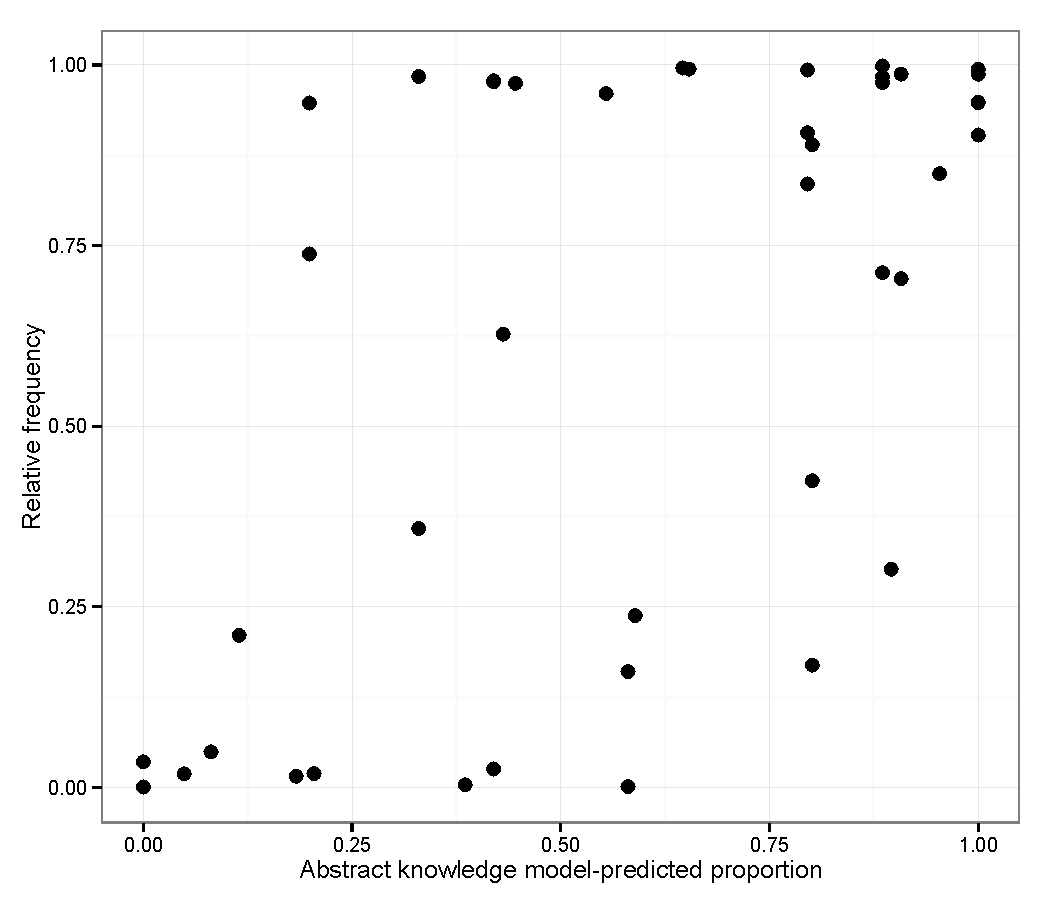
\includegraphics[scale=0.5]{model-by-freq.pdf}

\caption{Abstract knowledge model-predicted proportion and empirical relative frequency of each attested binomial appearing in alphabetical order. Abstract knowledge and relative frequency are significantly but not perfectly correlated.} 
\label{fig:model-by-freq}
\end{figure}

For our novel binomials, we chose expressions that our model predicts to have strong ordering preferences, with values less than 0.3 or greater than 0.7. As much as possible, we chose expressions that minimized the correlations between constraints (e.g. to dissociate length and frequency). A comparison of the profiles of constraint activity for novel and attested items is given in \ref{a:constraints}.


For all items, both novel and attested, we constructed a sentence context for the binomial expression, e.g.:
\begin{exe}
\item There were many bishops and seamstresses in the small town where I grew up.
\item There were many seamstresses and bishops in the small town where I grew up.
\end{exe}
Sentence structure was unrestricted, but the binomial expression was never in the first two or the last four words of the sentence. Sentences were designed not to introduce pragmatic constraints on binomial ordering: in particular, neither binomial element (nor any word related to exclusively or primarily to only one of the elements) was mentioned in the sentence before the binomial occurred.

With these materials, we carried out two behavioral experiments, a forced-choice preference experiment and a self-paced reading experiment.


\section{Experiment 1: Forced-choice preference}\label{expt1}
\subsection{Method}
\subsubsection{Participants}
75 native English speakers (mean age=36 years; sd=14) participated. Participants were recruited through Amazon Mechanical Turk, restricted to people connecting to the website from within the United States, and were paid 50 cents. Participants were asked to report their ``Native language (what you learned to speak with your mother as a child)''. Those who did not report English among their native languages were excluded.

\subsubsection{Procedure}
The Amazon Mechanical Turk instructions directed participants to an external website, where our experiment was presented using WebExp \citep{Keller:2009wn}. Participants first filled out a demographic questionnaire, then continued to the main experiment. On each trial, participants saw one item embedded in sentence context, in both possible orders, e.g.:
\begin{itemize}
\item There were many bishops and seamstresses in the small town where I grew up.
\item There were many seamstresses and bishops in the small town where I grew up.
\end{itemize}
Participants were asked to choose which order ``sounds more natural''. Each participant saw all 84 items. Which expression order was listed first was counterbalanced across participants. Order of item presentation was randomized separately for each participant. The experiment typically took 10-15 minutes.

\subsection{Results}
Before proceeding with multivariate analysis of the effects of abstract knowledge and direct experience on ordering preference, we present a striking overall difference between the distributions of preference strengths for attested versus novel binomials. Figure \ref{fig:judge} shows that ordering preferences are more polarized for attested than for novel binomials (despite the fact that we selected our novel binomials to have extreme preferences); in other words, preferences are more consistent across subjects for the attested expressions. We define a measure of extremity for each item as the difference between its experimentally determined preference strength (i.e. proportion of times preferred in alphabetical order) and 0.5. In a t-test, the attested items are significantly more extreme than the novel ($t=8.31, p < 0.001$). We discuss this issue further in Sections~\ref{fc-discuss} and~\ref{future-work}.

\begin{figure}[t]
\centering
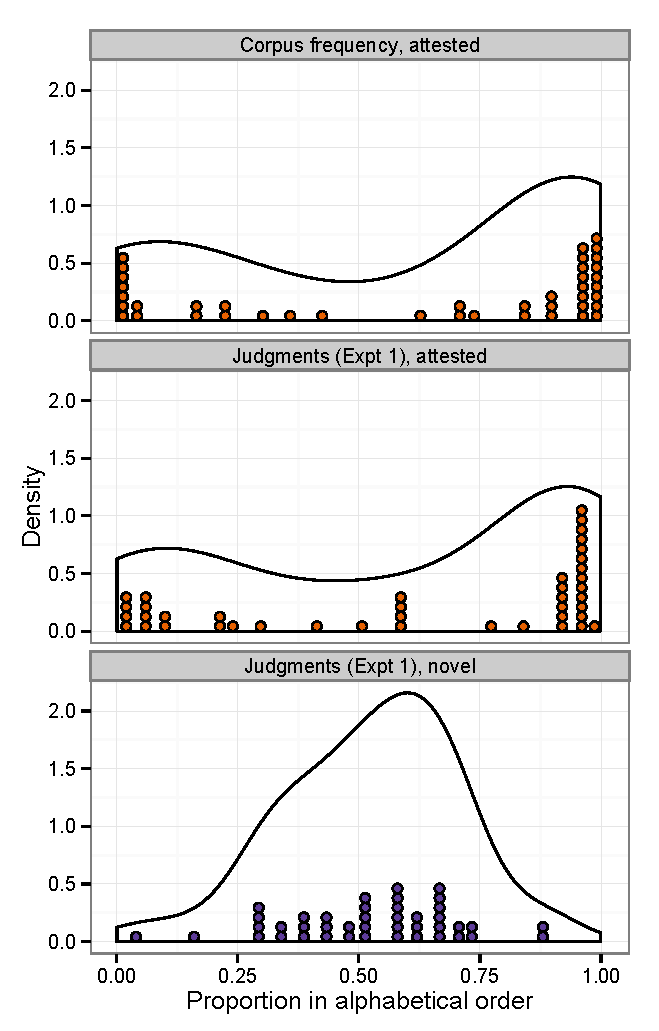
\includegraphics[scale=0.8]{just-judge-density-vertical.pdf}
\caption{Results of Experiment 1: Proportion of binomials occurring in alphabetical order in Google n-grams corpus frequency (top) and subjects' forced-choice preference judgments (middle/bottom). Dots show individual binomial types, while lines show density estimates. In judgments, attested binomials have more extreme preferences (i.e. more consistent across subjects) than novel binomials, demonstrating a qualitatively similar distribution to corpus frequencies.} \label{fig:judge}
\end{figure}

\subsubsection{Multivariate analysis}\label{expt1-multivariate}
Next we analyze our data using mixed-effects logistic regression \citep{TFlorianJaeger:2008ev}. Our dependent variable is the preferred order, coded as alphabetical or non-alphabetical: alphabetical order is used as a neutral order because results of our initial model selection---see Section \ref{model}---indicate that alphabetical order is not a significant predictor of ordering preference. Our independent (fixed-effect) predictors are:
\begin{itemize}
  \item \textbf{Type} (attested/novel) is treatment coded with ``attested'' as the reference level, i.e.\ the {\tt Intercept} value applies to attested items, and this value is adjusted by the {\tt Type:novel} value for novel binomials. We predict no significant intercept (i.e.\ attested binomials are not significantly more likely to be preferred in alphabetical or non-alphabetical order, absent other factors),  and no significant effect of type (i.e.\ novel binomials are not significantly more or less likely to be preferred in alphabetical order than attested binomials).
  \item  \textbf{Abstract knowledge} is operationalized as our model's predicted probability (between 0 and 1) of the expression occurring in alphabetical order. We center this predictor around 0.5. We nest the abstract knowledge predictor within type, i.e.\ we fit separate parameters for the effect of abstract knowledge for novel and attested binomials, allowing us to consider the effects of abstract knowledge on each type independently. For each type, if abstract ordering constraints are active in influencing offline judgments, then we predict a significant effect of abstract knowledge.
  \item \textbf{Relative frequency} estimates are computed for attested binomials using the Google n-grams corpus \citep{WebTgramVersio:tv} as the frequency of \emph{``A and B''} divided by the frequency of \emph{``A and B'' }plus \emph{``B and A''} (resulting in a value between 0 and 1), and centered around 0.5. Relative frequency for all novel binomials is set to 0 after centering. (Thus no interaction of relative frequency with type is necessary.) If direct experience with attested expressions influences offline judgments, then we predict a significant effect of relative frequency.
\end{itemize}
Following \citet{Barr:2013vf}, we use the maximal random effects structures for subjects and items justified by the experimental design: by-subject and by-item intercepts, and by-subject slopes for type, abstract knowledge, their interaction, and frequency.

Model results are given in Table \ref{t:fc-all}.\footnotemark{} Significance levels for effects are reported using the Wald $z$ statistic and are confirmed using likelihood ratio tests. We see a significant effect of abstract knowledge for both novel and attested expressions, demonstrating that abstract ordering constraints are active in determining forced-choice preferences for both binomial types. In a likelihood ratio test comparing this model to a model with only an additive (non-nested) fixed effect of abstract knowledge, we find no significant difference ($\chi^{2}(1)=1.63, p=0.20$); in other words, the effect of abstract knowledge does not differ significantly between novel and attested expressions. The effect of abstract knowledge for novel binomials is displayed in Figure \ref{fig:fc-abs}.

\footnotetext{The model presented here includes all the fixed-effect predictors and interactions that are of crucial theoretical interest for the hypotheses we set out to test. In order to explore possible further interactions between predictors, as well as possible changes in behavior over the course of the experiment, we fit a mixed-effects logistic regression including as predictors all the previous predictors, a trial order predictor, and all two-way interactions, using the {\tt MCMCglmm} package in {\tt R} \citep{Hadfield:uw}. (The trial order predictor was not included in the original model presented here because a main effect of trial order is implausible, as it would indicate a changing probability of prefering binomials in alphabetical order over the course of the experiment. However, its interaction with other predictors---in particular, abstract knowledge and relative frequency---is potentially of interest.) No further interactions (beyond the type x abstract knowledge interaction included in the original model) reached significance. }

We also see a significant effect of relative frequency, demonstrating that direct experience also plays a role in determining preferences for attested expressions. We note that relative frequency is a stronger predictor than abstract knowledge, measured in terms of larger regression coefficient estimate, larger $z$ value, and larger change in likelihood when removed from the model. The strong predictive power of relative frequency is displayed in Figure \ref{fig:fc-freq}. 


\begin{table}[t]
\centering
\begin{tabular}{ l  r  r  r  r  }
\hline\hline
 & \emph{Estimate} &\emph{Std. Error} & \emph{z value} & \emph{p value} \\   \hline
Intercept     &       -0.14 &    0.15  & -0.98& 0.33    \\  
Type: novel       &          0.25   &  0.19 & 1.32 &0.19 \\  
Abs know  (Type: attested)    &   2.32   &  0.56  & 4.12 & .00004^{***} \\  
Abs know (Type: novel)   &1.45 &    0.35  & 4.11 &.00004^{***}    \\  
Rel freq    &      6.18   &  0.49 & 12.55 & $<$2x10^{-16}^{***}\\\hline  
\end{tabular}
\caption{Model fit for results of Experiment 1. All VIF $< 1.2$. }\label{t:fc-all}
\end{table}


\begin{figure}[t]
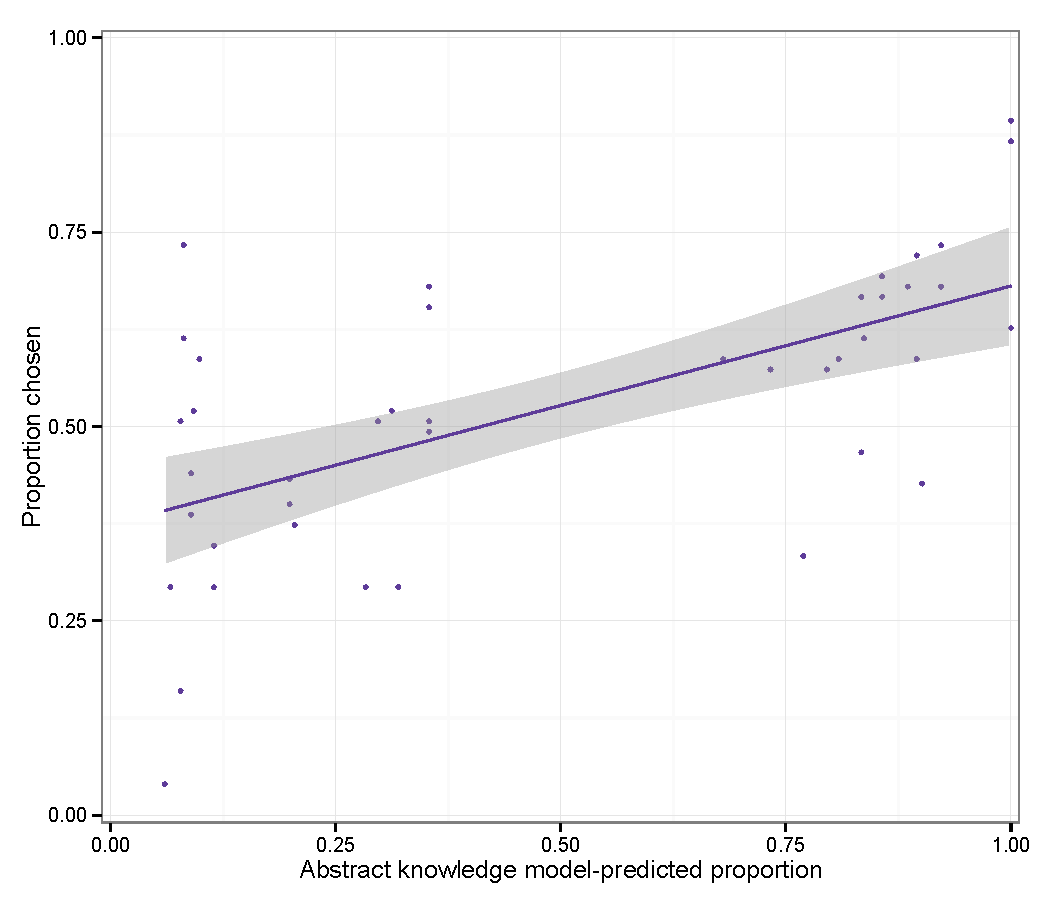
\includegraphics[scale=0.7]{fc-novel.pdf}
\caption{Results of Experiment 1 (novel items): Ordering preferences for novel binomials by model-predicted abstract knowledge. Each point represents an item. x values are the abstract knowledge model's prediction for how often the item will appear in alphabetical order. y values are how often the item was preferred in that order. Line shows best linear fit on the by-items aggregated data. Abstract knowledge is a significant predictor of preferences for novel expressions.} \label{fig:fc-abs}
\end{figure}

\begin{figure}[t]
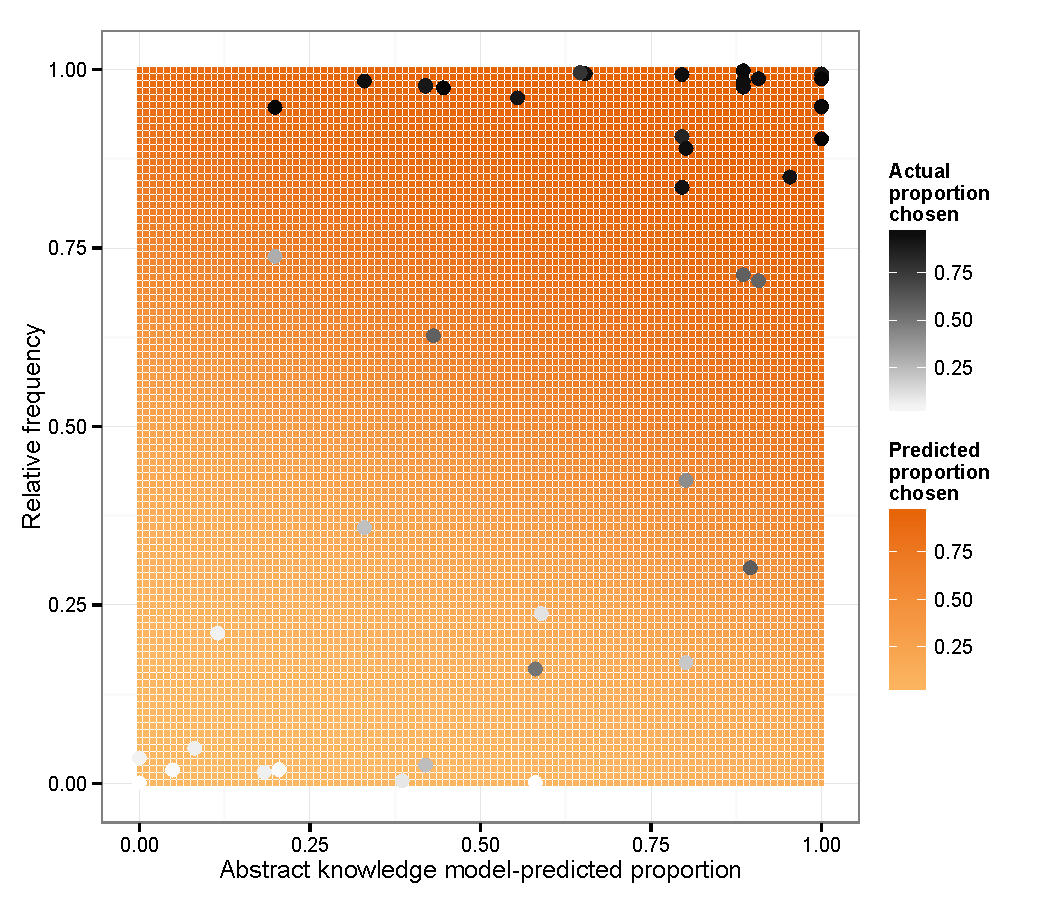
\includegraphics[scale=0.7]{fc-attested.pdf}

\caption{Results of Experiment 1 (attested items), visualized as colors overlaid on Figure \ref{fig:model-by-freq}. Each point represents an item. x values are the abstract knowledge model's prediction for how often the item will appear in alphabetical order. y values are the item's relative frequency of appearing in that order. Points' shading (white to black) shows often the item was preferred in that order. Background shading (light to dark orange) shows the best-fit model (Table \ref{t:fc-all}) prediction for how often the item was preferred in that order. Both relative frequency and abstract knowledge predict true preferences, as depicted by the diagonal background gradient but relative frequency is the stronger predictor, as depicted by the stronger vertical than horizontal gradient.} 
\label{fig:fc-freq}
\end{figure}

%The regression results, however, do not fully capture our qualitative impression of the data in Figure \ref{fig:fc-abs}. Visual inspection suggests that the results for attested binomials are more extreme than those for novel: that is, the datapoints cluster at the top and bottom of the y-axis, despite the model predictions being numerically (but not significantly) more extreme for the novel than for the attested items. (This pattern also produces the appearance of an interactive effect of type and abstract knowledge, although this interaction is not significant in our analysis.) We confirm this intuition by defining a measure of extremity for each item as its distance from 0.5 on the y-axis. In a t-test, the attested expressions are significantly more extreme than the novel ($t=8.31, p < 0.001$).

\subsection{Discussion}\label{fc-discuss}
In this experiment, we set out to test whether abstract knowledge and direct experience (specifically, relative frequency) predict ordering preferences in a forced-choice preference task for both novel and frequently attested binomial expressions. We demonstrate that preferences of both attested and novel expressions are affected by abstract knowledge and that preferences of attested expressions are also strongly predicted by relative frequency. This pattern of results supports a theory wherein both abstract knowledge and direct experience play a role in processing. Moreover, for attested expressions, we find that relatively frequency is a stronger predictor of preferences than abstract knowledge, suggesting that processing of these expressions relies more heavily upon direct experience than upon abstract knowledge. 

Although the effect of abstract knowledge does not differ significantly across binomial types, we do not think it is justified to draw strong theoretical conclusions from this null result. As we will see in Section \ref{multivariate}, abstract knowledge does interact significantly with binomial type in Experiment 2. We defer further discussion of this issue until Section \ref{exp2-dis}.

We additionally find that forced-choice preferences are more extreme for attested than for novel expressions; that is, attested expressions are more consistently preferred in one direction than novel expressions. Taken at face value, this finding suggests that increased overall frequency of an expression exaggerates or solidifies people's preferences. Another possibility, however, is that preferences for novel expressions are underlying equally as extreme as those of the attested expressions, but that the forced-choice judgement process for these items is noisier,\footnote{There are many reasons why this could be the case. For instance, when judging attested items, participants may believe that there is a ``right'' answer and take care to give that answer, whereas when judging novel items, they may put in less effort.} making the resulting preferences for novel expressions appear less extreme than they truly are. We will return to this question in the general discussion.

One potential confound mentioned earlier is the role of local sentence context on binomial order preferences. Although we tried to avoid biasing contexts in designing our materials, it is always possible that some bias unintentially slipped through. Thus we hasten to point out that even if such bias does exist within individual sentences---i.e. the sentence context favors one order more than another, relative to the binomials' intrinsic ordering preference in a hypothetical neutral context---it would not confound the results presented here. Specifically, because our dependent variable is an alphabetical versus non-alphabetical preference, in order to bias our results the local context biases would need to be systematically correlated with the alphabetical/non-alphabetical preferences as given by our predictors of interest (abstract knowledge and relative frequency). Since we have no reason to expect this to be the case, any unintentional effects of local context will merely add noise to our estimates of ordering preferences.

In the next experiment, we ask whether the patterns found in our forced-choice preference experiment likewise hold in an online reading experiment.


\section{Experiment 2: Self-paced reading}\label{expt2}
\subsection{Method}
\subsubsection{Participants}
400 native English speakers (mean age=34 years; sd=12) participated.\footnote{Experiment 2 required substantially more participants than Experiment 1 because the self-paced reading data is noisier than the forced-choice data, and because each subject saw approximately half the items in Experiment 2 (compared to all the items in Experiment 1).} Participant recruitment was identical to Experiment 1, except that participants were paid \$1.00.

\subsubsection{Procedure}
The experiment was presented within Amazon Mechanical Turk using flexspr (\citealp{flexspr:cFpvxjkw}; previously used by \citealp{Bergen:2012ur,Singh:2015uf}). Using this method online allows for collection of more data than would be possible in a laboratory setting, and previous work has replicated multiple in-the-lab results with web-based self-paced reading \citep{Enochson:2015dy}. Participants first filled out a demographic questionnaire, then read sentences in a self-paced reading paradigm: sentences were presented one word at a time, and participants pressed a button to advance to the next word. Reading times for each word were recorded. Participants read three practice sentences, then continued to the main experiment.

Our materials consisted of the same 84 binomial expressions in sentence context as used in Experiment 1, plus 84 unrelated filler sentences. Two stimulus lists were constructed with items rotated and counterbalanced between lists so that each participant only saw a given binomial in one of its two possible orders. Due to a programming error, out of the 168 items in each list, each participant saw a random selection of 80 items. Order of presentation was randomized separately for each participant.

Presentation of each sentence was followed by a yes/no comprehension question. Answers did not depend on the order of the binomial expression. The experiment typically took about 30 minutes.


\subsection{Results}

\subsubsection{Comprehension question accuracy}
Comprehension question accuracy is extremely high across all conditions. See Table \ref{t:qcorrect}.


\begin{table}[t]
\centering
\begin{tabular}{ccc}\hline\hline
& novel & attested \\\hline
preferred & 0.97 & 0.97 \\
non-preferred & 0.97 & 0.96 \\\hline
\end{tabular}
\caption{Comprehension question accuracy for Experiment 2. Novel and attested items are divided into preferred/non-preferred order according to abstract knowledge model predictions.}\label{t:qcorrect}
\end{table}

\subsubsection{Multivariate analysis}\label{multivariate}
We use regression analysis to compare abstract knowledge and relative frequency as predictors of reading times, analagous to our analysis in Experiment 1.

We divide our experimental items into regions of analysis as shown below:

\noindent\begin{tabular}{c c c c c c c c c c}
 \emph{Prelim} & \emph{Word1} & \emph{And} & \emph{Word2} & \emph{Spill1} & \emph{Spill2} & \emph{Spill3 } & \\
\multirow{2}{*}{There were many} & bishops & \multirow{2}{*}{and} & seamstresses & \multirow{2}{*}{in} & \multirow{2}{*}{the} & \multirow{2}{*}{small} & \multirow{2}{*}{\ldots}\\
&seamstresses&&bishops
\end{tabular}

\noindent The \emph{Prelim} region encompasses the entire beginning of the sentence up to the binomial expression; all further regions are a single word. We analyze reading time data for each trial summed over a six-word region spanning from Word1 through Spill3. By summing across reading times for these regions, we take advantage of the controlled properties of our stimuli: regardless of order of binomial presentation across conditions, participants will have read the same group of words within the region being analyzed. (For more direct comparison with the previous literature, we present word-by-word analyses of reading times in \ref{word-by-word}.)

Specifically, we computed a summed reading time measure for each trial as follows: we excluded all trials in which the reading time for any word was less than 100ms or greater than 5000ms (following \citealp{Fine:2013vt}). To account for influences of word length, as described by \citet{Ferreira:1986vz}, we then computed subject-specific residualized reading times (regressed against word length) for each word from the Word1 through Spill3 regions, using data from all non-sentence-final words in non-practice trials.\footnote{For analyses using raw reading times, see \ref{raw-rts}.} Summing the residuals for this six-word region gives us a residual reading time for each trial. We performed outlier removal without regard to item type or condition: we computed a grand mean and standard deviation and exclude trials with summed times more than 2.5 standard deviations above or below the mean (following \citealp{Garnsey:1997vo}), resulting in a loss of 1.7\% of data.

We analyze the data using a mixed-effects linear regression similar to that used in Experiment 1. Our dependent variable is summed residual reading time. Our independent (fixed-effect) predictors and their interpretations are identical to those used in Experiment 1 (Section \ref{expt1-multivariate}) with one addition:
%
\begin{itemize}
  \item \textbf{Trial order} is the position in the experiment in which the given trial occurred. As is common in reading experiments (e.g. \citealp{Hofmeister:2011vg,Fine:2013vt} and many others), we expect that subjects will read faster later in the experiment due to practice effects.
\end{itemize}
%
In addition to our hypotheses regarding possible influences of abstract knowledge and direct experience on reading times (which are the same as in Experiment 1), we additionally anticipate a possible statistically significant but theoretically uninteresting main effect of binomial type because the two types contain different words in different sentence frames, and thus one type may be read faster than the other. Following \citet{Barr:2013vf}, we use the maximal random effects structure for subjects as justified by the experimental design, namely an intercept and slopes for type, abstract knowledge, their interaction, and relative frequency. We also include a by-subjects random slope for trial order. For items, defined as unordered word pairs, we include a random intercept, a random slope for trial order, and (in place of random slopes for both abstract knowledge and relative frequency) a random slope for a binary alphabetical/non-alphabetical factor, thus allowing for arbitrary item-specific ordering preferences.


Model results are given in Table \ref{t:spr-all}.\footnotemark{} Effects with $t\ge 2$ are taken to be significant. Positive coefficients indicate slower reading. We see a significant main effect of type with novel expressions read slower, which we attribute to these expressions containing less frequent words on average, in addition to being less frequent expressions overall.

\footnotetext{The model presented here includes all the fixed effect predictors and interactions that are of crucial theoretical interest for the hypotheses we set out to test. In order to explore possible further interactions between predictors, we fit a mixed-effects linear regression including as predictors all these fixed-effect predictors and all two-way interactions using the {\tt MCMCglmm} package in {\tt R} \citep{Hadfield:uw}. No further interactions (beyond the type x abstract knowledge interaction included in the original model) reached significance.}

We do not find a significant effect of abstract knowledge for attested expressions, suggesting that abstract ordering constraints are not active in the online processing of these expressions. However, we do find a significant effect of abstract knowledge for novel expressions. In a likelihood ratio test comparing this model to a model with only an additive (non-nested) effect of abstract knowledge, we find a significant difference ($\chi^{2}(1)=4.24, p<0.04$); in other words, the effect of abstract knowledge differs significantly between novel and attested expressions, playing a significant role in online processing for novel expressions only.
We additionally find a significant effect of relative frequency, demonstrating that higher relative frequency leads to faster reading in the online processing of attested expressions. 

Finally, we find a significant effect of trial order, with faster reading later in the experiment. Results are visualized in Figures \ref{fig:spr-model} and \ref{fig:spr-freq}.

\begin{table}[t]
\centering
\begin{tabular}{ l  r  r  r  }
\hline\hline
 & \emph{Estimate} &\emph{Std. Error} & \emph{t value}  \\\hline    
Intercept   &  196.34   &  26.04   & 7.54\\ 
Type: novel & 195.17 &    25.77  & 7.57\\ 
Abs know (Type: attested)      &   13.88    & 23.14  &  0.60\\ 
Abs know (Type: novel) & -48.73 &     18.02 &  -2.70 \\ 
Rel freq &  -59.25  &   18.42  & -3.22\\ 
Trial order &           -8.35   &   0.39 & -21.24\\\hline 
\end{tabular}
\caption{Model fit for results of Experiment 2. Effects with $t>2$ are taken to be significant. All VIF $< 1.7$.}\label{t:spr-all}
\end{table}


\begin{figure}[t]
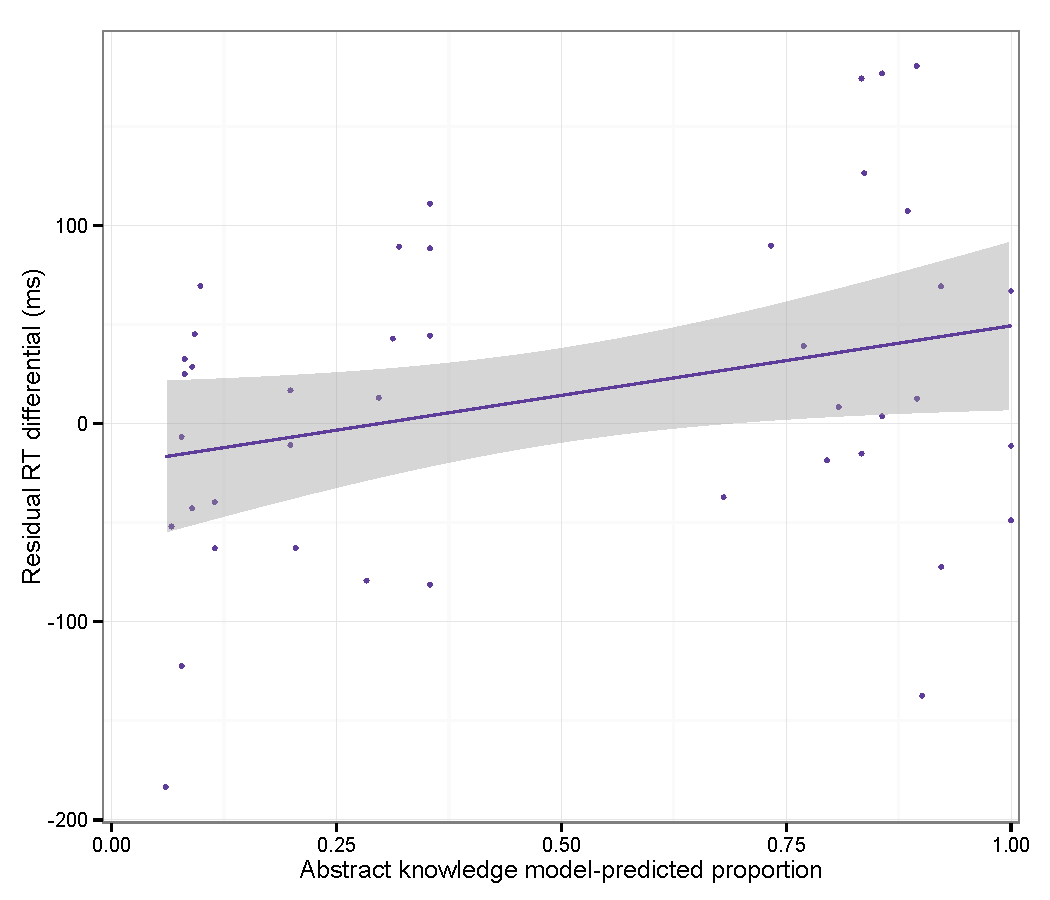
\includegraphics[scale=0.87]{spr-results.pdf}
\caption{Results of Experiment 2 (novel items): Reading time differentials for novel binomials by model-predicted abstract knowledge. Each point represents an item. x values are abstract knowledge model's predictions for how often the item will appear in alphabetical order. y values are the differences between average summed residual reading times for the non-alphabetical and alphabetical orders. Line shows best linear fit on the by-items aggregated data. Abstract knowledge is a significant predictor of reading times.} \label{fig:spr-model}
\end{figure}


\begin{figure}[t]
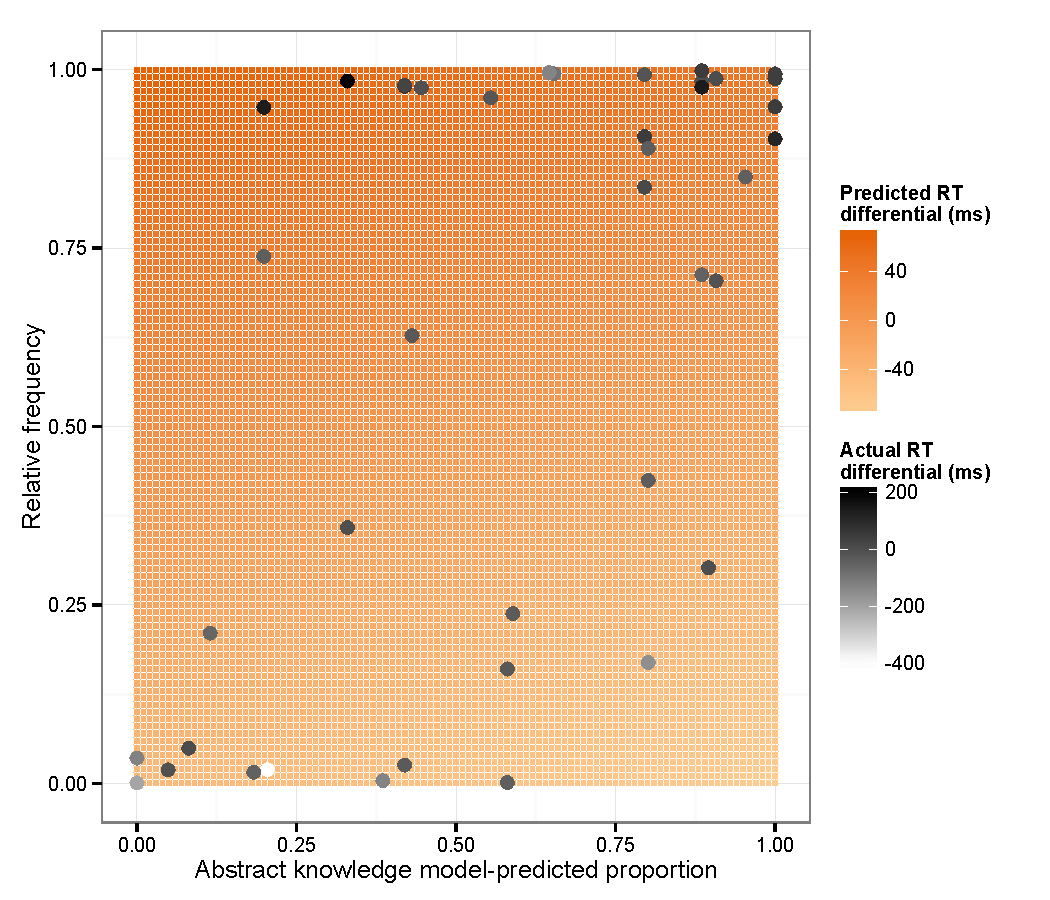
\includegraphics[scale=0.7]{spr-attested.pdf}
\caption{Results of Experiment 2 (attested items), visualized as colors overlaid on Figure \ref{fig:model-by-freq}. Each point represents an item. x values are the abstract knowledge model's prediction for how often the item will appear in alphabetical order. y values are the item's relative frequency of appearing in that order. Points' shading (white to black) shows the item's true average RT differential. Background shading (light to dark orange) shows the best-fit model (Table \ref{t:spr-all}) prediction for RT differential. Only relative frequency is a significant predictor of reading times, as depicted by the strong vertical background gradient.} \label{fig:spr-freq}
\end{figure}

\subsection{Discussion}\label{exp2-dis}
We demonstrate for the first time that novel binomial expressions show online effects of abstract ordering preferences. In contrast, reading times for frequently attested binomial expressions are only influenced by relative frequency. These findings imply a trade-off in online processing between reliance on abstract knowledge and direct experience, where novel expressions must be processed on the basis of abstract knowledge only, but highly frequent attested expressions can be processed primarily with reference to previous direct experience.

Here we found a significant interaction of abstract knowledge with binomial type, such that abstract knowledge was significantly less active in determining reading times for attested binomials than for novel binomials. In contrast, in Experiment 1, we found no such significant interaction. What is consistent across these two experiments is that processing of attested expressions is more strongly influenced by direct experience than by abstract knowledge. However, given the inconsistent results concerning the interaction of abstract knowledge and binomial type, we cannot state with confidence whether abstract knowledge is differentially active between novel and attested binomials.

\section{General discussion}\label{discussion}

We set out to investigate the roles of abstract knowledge and direct experience in the processing of binomial expressions, asking whether binomial ordering preferences are driven by constraints on the semantic, phonological, and lexical properties of words in an expression, or by prior experience with the specific expression in question. Our key findings are as follows. First, we demonstrated that abstract ordering constraints are active in the comprehension of novel expressions in both an offline forced-choice task and a online self-paced reading task. Second, we demonstrated that for frequently attested expressions, effects of direct experience largely overwhelm abstract knowledge in predicting behavioral data, both in the offline task and especially in the online task.

Our results support exemplar- or usage-based theories of language, which allow for the storage and reuse of multi-word expressions. Specifically, our finding that ordering preferences for attested binomial expressions are primarily driven by relative frequency is evidence that the processing of these expressions makes use of holistic multi-word mental representations. In contrast, a traditional words-and-rules theory would predict that these expressions are generated compositionally each time they are encountered, and that the ordering preferences of attested expressions, like those of novel expressions, should stem from abstract ordering constraints rather than relative frequency of direct experience.

%Our investigation addresses two previous limitations in the study of the processing of frequent multi-word expressions. First, our choice of materials avoid confounds due to real-world plausibility differences because the meaning of binomial expressions is not changed by the order of the elements within the compound. Second, our experimental design allows for quantitative comparisons between abstract knowledge and direct experience: our probabilistic model provides quantitative estimates for the effects of abstract knowledge, while corpus frequencies provide estimates for direct experience. Using regression modeling, we can directly compare the predictive strength of these two influences.

Of the predictions made in Section \ref{predictions}, our results indicate that both abstract knowledge and relative frequency play a role in the processing of binomial expressions. Many patterns are possible for the manner in which these two knowledge sources trade off as a function of the overall frequency of an expression: In one extreme, abstract knowledge could apply only for expressions that have never before been encountered, with relative frequency taking over as soon as any direct experience exists. In the other extreme, abstract knowledge could apply in the vast majority of cases, with relative frequency limited to playing a role only for the highest frequency items, such as those used in our experiments. A middle ground position proposes a gradual switch from reliance on abstract knowledge to reliance on relative frequency as overall frequency increases.

We propose that both extremes are unlikely and that the middle position of a gradual trade-off is the most likely. The first extreme is counterintuitive, since a single encounter with an expression seems insufficient to thoroughly trump abstract knowledge. The second extreme has been argued against by \citet{Arnon:2010hz}, who found frequency effects for multi-word expressions across a wide range of frequencies. Their finding of frequency effects for low-to-medium frequency items would not be predicted by a theory in which direct experience applies only to the processing of extremely high frequency items. The gradual trade-off theory, on the other hand, is supported by a wide variety of computational models.

\subsection{Convergent evidence from computational models}
\subsubsection{Connectionist models}
A similar trade-off has been demonstrated in connectionist models of language learning in domains such as past-tense formation \citep{Rumelhart:1986wx} and grammatical structure \citep{Elman:2003vo}, which learn both generalized patterns and specific exceptions. These models learn to predict patterns within their training data (e.g. Form the past tense by adding \emph{-ed}). When new items are introduced, they are at first treated accorded to the general patterns, but with further training, the model can learn to treat certain items as exceptions.

These models have primarily been conceived as models of early language acquisition and tested on frequent items (e.g. common verbs), where it can assumed that by adulthood, most native speakers will have extensive experience with all the items in questions, and will thus consistently recognize certain words as exceptions to the general rules. However, their behavior on new items straightforwardly generalizes to low frequency items that even adult native speakers would have relatively little direct experience with, such as attested but low frequency binomial expressions, making the prediction that these items could occupy a middle ground of partial reliance upon both general patterns (i.e. abstract knowledge) and direct experience, even in a fully developed adult grammar.


\subsubsection{Exemplar-based computational models}
A gradual trade-off is also predicted by exemplar-based computational models of language \citep[e.g.][]{Bod:1998tx,Bod:2003uw, Bod:2008uc, Johnson:2007wl, Demberg:2010tf, ODonnell:2011vh}. These models---which primarily focus on adult-like language representation, rather than acquisition---incorporate representations of sentence fragments of varying sizes, thus allowing for the representation of holistic multi-word expressions as well as the individual words and rules used to generate such expressions compositionally. Within these models, multi-word expressions can thus be parsed both through direct reuse and through compositional generation. The probabilities assigned to these units---the holistic expressions, the individual words, and the compositional rules---will collectively determine the relative likelihoods of reuse versus regeneration. For more frequent expressions, the probability of reusing a holistic unit will be higher, while for less frequent expressions, the probability of compositional generation will be higher. These probabilities change gradually depending on the frequency of a given expression as well as the frequencies of similar expressions. These models thus also predict a gradual trade-off between reliance on abstract knowledge for infrequent items and reliance upon direct experience for frequent items.

\subsubsection{Nonparametric Bayesian models}
The gradual trade-off theory is also supported by a nonparametric Bayesian perspective \citep[e.g.][]{Goldwater:2009jy,Xu:2007dt}, in which expectations are influenced by both a prior probability and the incoming data. In a Bayesian model, when little data has been seen, expectations are driven by the prior probability. As more data is seen, the data becomes increasingly influential, asymptotically approaching complete dominance. For binomial expressions, abstract knowledge can be thought of as a prior probability for ordering preferences, absent any direct experience with a given expression, and each direct encounter with an expression constitutes further data. Under the Bayesian perspective, when one has little experience with an expression, expectations will be governed by abstract knowledge, but with increasing experience, the relative frequency of ordering within the experienced data will be increasingly dominant in determining expectations.

\subsection{Advantages of our approach}
While numerous models support our conclusions, the experiments presented here crucially advance the state of our understanding beyond what was previously known by providing a novel approach for using \emph{behavioral evidence}, in conjunction with modern corpora and multivariate statistics, to quantify the contributions of abstract knowledge and direct experience. Our probabilistic model provides quantitative estimates for the effects of abstract knowledge, while corpus frequencies provide estimates for direct experience. Using multivariate regression modeling, we can directly compare the predictive strength of these two influences on behavioral data such as the results of our forced-choice and self-paced reading tasks. This approach allows us to move beyond the previous modeling-based approaches, which focused on predicting corpus data or language-wide trends. We can now investigate the trade-off between abstract knowledge and direct experience using behavioral evidence.

Additionally, the statistical techniques employed here allow us to make quantitative claims about the strength of reliance on both abstract knowledge and direct knowledge. We have seen this in a limited way so far, as we demonstrated that processing of frequently attested binomials is driven primarily by relative frequency, and only to a lesser degree by abstract knowledge. We have also predicted that there should be a gradual shift from reliance upon abstract knowledge to reliance upon relative frequency estimates as overall frequency increases; however, we cannot conclude this directly from our current data because overall frequency has only been explored as a dichotomous variable: either entirely novel or very frequent. In future work, we plan to look at an in-between zone of attested but not highly frequent expressions, e.g. \emph{sunglasses and sunscreen}/\emph{sunscreen and sunglasses} ($1/1000$th the frequency of the average attested expression in the current study). We predict that these expressions should show noticeable effects of both abstract constraints and relative frequency. Moreover, looking over a range of overall frequencies, we predict that we will see a quantitative trade-off between reliance on abstract knowledge and reliance on direct experience. 

This approach to studying the trade-off between abstract knowledge and direct experience generalizes beyond the study of binomial expression ordering preferences. The cornerstone of this approach is that we are able to independently quantify the contributions of direct experience with specific expressions and abstract knowledge in the absence of direct experience. We propose that a combination of corpus frequencies and probabilistic modeling can provide such estimates for a wide range of linguistic constructions (e.g. the dative alternation [\citealp{Bresnan:2007td}] and adjective ordering [\citealp{Dixon:1982ur, Truswell:2009cr}]) allowing us to ask broad questions about the trade-off between compositional generation and the reuse of stored expressions in linguistic processing. For example, to what extent are adjective ordering preferences due to abstract rules (e.g. shape before color) versus to known collocations of highly frequent adjective sequences? The methods we have developed here make these questions accessible for future research.

\subsection{Further predictions about language structure}\label{future-work}

Our results additionally lead to predictions about language structure. Our gradual trade-off theory predicts that items with higher overall frequency will be more likely to have relative frequency preferences that contradict abstract knowledge preferences. This prediction is analogous to the finding that more frequent verbs are more likely to be irregular \citep{Lieberman:2007bl}: in the case of high overall-frequency items, people have enough exposure to learn idiosyncratic or abstract-knowledge-violating preferences, but in the case of low overall-frequency items, people have insufficient exposure to overcome their abstract knowledge. A further prediction follows from the results of Experiment 1, in which we found that preferences for attested items were more extreme, or polarized, than preferences for novel items. Assuming that preferences for attested items are driven primarily by relative frequency, this result predicts that as overall frequency increases, relative frequencies will become more polarized.\footnote{We did not see the analog of this result in Experiment 2: reading time were not slower in the dispreferred order and faster in the preferred order for attested than for novel expressions. Based on the results of \citet{Morgan:2015to}, we conclude that this is due either to noise or to floor/ceiling effects on reading times.}

In related work, we found that these predictions were borne out in a corpus analysis \citep{Morgan:2015to}, which demonstrated that binomial expressions with higher overall frequency have relative frequencies that deviate more from abstract knowledge---in particular, by being more polarized. This finding in turn leads to further questions about the historical trajectories of binomial expression ordering preferences, and the dual roles of individuals' language processing and cultural transmission in shaping language structure \citep{Anonymous:GVZA8N7s}. Thus the results presented here additionally open the door to further investigation of the mutually constraining processes of synchronic language processing and diachronic language change.





%\section{Conclusion}
%We investigate the roles of abstract knowledge and direct experience in the processing of binomial expressions such as \emph{bread and butter}. In two behavioral experiments, we find that processing of novel expressions is affected by abstract constraints that reference phonological, semantic, and lexical properties of their elements, whose effects we estimate using a probabilistic model. In contrast, processing of frequently attested expressions is primarily driven by direct expression-specific experience. Our findings demonstrate that abstract ordering constraints are active in the online processing of binomial expressions, and support exemplar-based models of language which claim that multi-word expressions can be stored and processed as holistic units.

\section*{Acknowledgements}
This work has benefited from presentation and discussion at a variety of venues, including the 26th annual CUNY Sentence Processing Conference and the 2014 annual meeting of the Linguistic Society of America. Thank you to Inbal Arnon, Grant Goodall, and an anonymous reviewer for helpful discussion, to Mike Brooks for assistance with preparation of experimental materials and data coding, and to Harry J. Tily for providing us with flexspr. The research presented here was funded by research grants NSF 0953870 and NICHD R01HD065829 and fellowships from the Alfred P. Sloan Foundation and the Center for Advanced Study in the Behavioral Sciences to Roger Levy, and NIH T32-DC000041 to the UCSD Center for Research in Language.

\appendix
\section{Experimental materials}
Comprehension questions are used only in Experiment 2.

\subsection{Novel expressions}

\begin{enumerate}
\item He was \textbf{abashed} and \textbf{sorry} about his horrible behavior.	\begin{itemize} \item Did he defend his behavior?\end{itemize}
\item This bar is popular among the \textbf{actresses} and \textbf{lumberjacks} who live in the neighborhood.	\begin{itemize} \item Do the lumberjacks hate the bar?\end{itemize}
\item Because Jim was \textbf{allergic} and \textbf{unaccustomed} to elderberries, he was careful to avoid them.	\begin{itemize} \item Did Jim like to eat elderberries?\end{itemize}
\item My cousin's new talking and singing toy is \textbf{annoying} and \textbf{teal} according to my aunt.	\begin{itemize} \item Does my cousin have a new toy?\end{itemize}
\item The dentist told Sally that \textbf{bacteria} and \textbf{candy} would rot her teeth.	\begin{itemize} \item Did the dentist recommend eating candy?\end{itemize}
\item The elephants at the zoo were \textbf{beautiful} and \textbf{stinky} so the children loved them.	\begin{itemize} \item Were there elephants at the zoo?\end{itemize}
\item The engineer specialized in making \textbf{bicycles} and \textbf{robots} when he worked for the company.	\begin{itemize} \item Did the engineer specialize in destroying things?\end{itemize}
\item There were many \textbf{bishops} and \textbf{seamstresses} in the small town where I grew up.	\begin{itemize} \item Did I grow up in a small town?\end{itemize}
\item The berries were \textbf{bitter} and \textbf{purple} when I ate them this morning.	\begin{itemize} \item Did I eat berries this morning?\end{itemize}
\item Seth told me that there are \textbf{blankets} and \textbf{kittens} in that box over there.	\begin{itemize} \item Were there blankets in the box?\end{itemize}
\item The rangers seemed to act like \textbf{campfires} and \textbf{wildfires} were the same thing.	\begin{itemize} \item Did I hear about fires from a policeman?\end{itemize}
\item At the wizard school, \textbf{chanting} and \textbf{enchanting} were very common occurrences.	\begin{itemize} \item Did the wizards ride broomsticks frequently?\end{itemize}
\item When I met many \textbf{chauffeurs} and \textbf{stewardesses} at a party, I started questioning my job.	\begin{itemize} \item Did I go to a party?\end{itemize}
\item The third grade class saw \textbf{cherries} and \textbf{llamas} at the state fair.	\begin{itemize} \item Did the class go to the state fair?\end{itemize}
\item There was nothing but \textbf{chickens} and \textbf{fences} in the field behind the house.	\begin{itemize} \item Was the field behind the house?\end{itemize}
\item His uncles were all \textbf{coroners} and \textbf{senators} in their day jobs, but they all wanted to get into the movie industry.	\begin{itemize} \item Did he have uncles?\end{itemize}
\item The drink flavored with \textbf{currant} and \textbf{pomegranate} was delicious according to Kim.	\begin{itemize} \item Did Kim like the drink?\end{itemize}
\item The dictator was \textbf{deposed} and \textbf{murdered} by his military adviser.	\begin{itemize} \item Did the dictator survive?\end{itemize}
\item I talked with my boss about whether to hire the \textbf{determined} and \textbf{forgettable} job candidate that we interviewed.	\begin{itemize} \item Did I discuss something with my boss?\end{itemize}
\item The doctor said that \textbf{discontent} and \textbf{tearfulness} are signs of depression.	\begin{itemize} \item Did the doctor talk about flu symptoms?\end{itemize}
\item Luke always looked so \textbf{disheveled} and \textbf{dreary} but he was my best friend.	\begin{itemize} \item Was Luke my best friend?\end{itemize}
\item The kind minister \textbf{donates} and \textbf{provides} a lot of food to the charity.	\begin{itemize} \item Was the minister kind?\end{itemize}
\item My favorite animals have been \textbf{felines} and \textbf{quails} ever since I was a kid.	\begin{itemize} \item Have I always hated animals?\end{itemize}
\item The finalists in the tennis championship were ranked \textbf{first} and \textbf{ninety-eighth} in the world prior to the tournament.	\begin{itemize} \item Was there a golf champtionship?\end{itemize}
\item In the spring, Julie will plant \textbf{flowers} and \textbf{zinnias} in her new garden.	\begin{itemize} \item Does Julie have a garden?\end{itemize}
\item The store owner was \textbf{fuming} and \textbf{mad} when he found out what was stolen.	\begin{itemize} \item Was something stolen?\end{itemize}
\item As a vegetarian, \textbf{gelatin} and \textbf{lard} are difficult to avoid.	\begin{itemize} \item Do vegetarians have a hard time?\end{itemize}
\item Laura heard that the school's \textbf{groundskeeper} and \textbf{superintendent} got married over the summer.	\begin{itemize} \item Did Laura hear about a divorce?\end{itemize}
\item His mother didn't hear when when Nate \textbf{happily} and \textbf{rudely} told his sister to shut up.	\begin{itemize} \item Did his mother hear what Nate said?\end{itemize}
\item As Joe carried a tall stack of boxes, he had to \textbf{hesitate} and \textbf{readjust} before he could go further.	\begin{itemize} \item Was the worker carrying barrels?\end{itemize}
\item At the zoo we saw \textbf{horses} and \textbf{loons} in their natural habitats.	\begin{itemize} \item Did we go to the zoo?\end{itemize}
\item I need to grab my \textbf{jacket} and \textbf{phone} before I leave the house.	\begin{itemize} \item Do I have everything I need in order to leave?\end{itemize}
\item Sarah likes to buy \textbf{kale} and \textbf{vegetables} at the famer's market.	\begin{itemize} \item Does Sarah only buy meat?\end{itemize}
\item My cousins were all \textbf{lankier} and \textbf{lanky} but were surprisingly strong.	\begin{itemize} \item Were my cousins weak?\end{itemize}
\item The pet store was full of \textbf{litter} and \textbf{newts} when Martha visited on Saturday.	\begin{itemize} \item Did Martha go to the pet store?\end{itemize}
\item Peter met a man who was \textbf{masculine} and \textbf{undignified} at the conference he went to last month.	\begin{itemize} \item Did Peter go to the conference last year?\end{itemize}
\item The pirate was \textbf{marooned} and \textbf{missing} for nearly five months.	\begin{itemize} \item Was the pirate stranded for a year?\end{itemize}
\item My grandparents were all \textbf{nurses} and \textbf{patriarchs} when they were alive.	\begin{itemize} \item Were some of my grandparents teachers?\end{itemize}
\item In my dream, I had \textbf{puppies} and \textbf{tigers} that I kept as pets.	\begin{itemize} \item Was I dreaming?\end{itemize}
\item Jenny was interested in \textbf{rats} and \textbf{sharks} as a young child.	\begin{itemize} \item Was Jenny interested in kittens?\end{itemize}
\item Maria could use \textbf{therapy} and \textbf{vacations} to feel less stressed.	\begin{itemize} \item Is Maria stressed?\end{itemize}
\item Irena had trouble with \textbf{vocabulary} and \textbf{vowels} while she was learning English.	\begin{itemize} \item Did Irena have trouble with vowels?\end{itemize}\end{enumerate}

\subsection{Attested expressions}

\begin{enumerate}

\item The clerk asked for Melissa's \textbf{address} and \textbf{name} in order to complete the form.	\begin{itemize} \item Did the clerk help Melissa complete the form?\end{itemize}
\item Sarah was relieved to find that her friends were \textbf{alive} and \textbf{well} after the car crash.	\begin{itemize} \item Were Sarah's friends alright?\end{itemize}
\item Most universities have programs in the \textbf{arts} and \textbf{sciences} in addition to having various professional schools.	\begin{itemize} \item Do most university have programs about law?\end{itemize}
\item Soccer players practice running both \textbf{backwards} and \textbf{forwards} in order to stay nimble.	\begin{itemize} \item Do soccer players practice running sideways?\end{itemize}
\item Hunter dislikes reading \textbf{black} and \textbf{white} text off a computer screen so he uses an unusual color scheme.	\begin{itemize} \item Does Hunter like the standard color scheme?\end{itemize}
\item Learning to strengthen your \textbf{body} and \textbf{mind} is one of main purposes of doing yoga.	\begin{itemize} \item Does yoga improve your strength?\end{itemize}
\item George always brings \textbf{bread} and \textbf{butter} with him when he goes camping.	\begin{itemize} \item Does George always bring hot chocolate when he goes camping?\end{itemize}
\item John showed me pictures of the \textbf{bride} and \textbf{groom} both dressed in blue.	\begin{itemize} \item Did the couple wear green?\end{itemize}
\item I always love seeing my \textbf{brothers} and \textbf{sisters} when I go home for the holidays.	\begin{itemize} \item Do I enjoy going home?\end{itemize}
\item Caleb likes to \textbf{buy} and \textbf{sell} electronics on eBay as a hobby.	\begin{itemize} \item Does Caleb work with eBay professionally?\end{itemize}
\item I watched the \textbf{cat} and \textbf{mouse} run frantically around the barn.	\begin{itemize} \item Was there a dog in the barn?\end{itemize}
\item It can be difficult to determine the \textbf{cause} and \textbf{effect} of weather patterns over the ocean.	\begin{itemize} \item Are ocean weather patterns hard to predict?\end{itemize}
\item Clarissa found the painting of a \textbf{child} and \textbf{mother} to be very moving.	\begin{itemize} \item Did Clarissa see a painting?\end{itemize}
\item Catherine was not surprised that tensions between \textbf{church} and \textbf{state} ran high during the election season.	\begin{itemize} \item Was there tension during the election season?\end{itemize}
\item Peter studied the laws concerning \textbf{crime} and \textbf{punishment} in Ancient Greece and Rome.	\begin{itemize} \item Did Peter study what happened in Ancient Greece?\end{itemize}
\item Jesse felt like he had worked \textbf{day} and \textbf{night} on the project but he only got a B on it.	\begin{itemize} \item Did Jesse get an A?\end{itemize}
\item The economist became famous for studying the way \textbf{demand} and \textbf{supply} affect the steel industry.	\begin{itemize} \item Did the economist study oil companies?\end{itemize}
\item Mark finds working on \textbf{development} and \textbf{research} for the marketing company to be a very satisfying career.	\begin{itemize} \item Does Mark want to change jobs?\end{itemize}
\item Although some \textbf{drink} and \textbf{food} were provided at the reception, there was not enough to go around.	\begin{itemize} \item Was there something to eat at the reception?\end{itemize}
\item Diane wrote a book about her travels \textbf{east} and \textbf{west} around the globe for a year.	\begin{itemize} \item Did Diane write a book about living in Paris?\end{itemize}
\item Sometimes it feels like \textbf{error} and \textbf{trial} is the only way to learn.	\begin{itemize} \item Do you sometimes need to learn by trying things?\end{itemize}
\item Heather invited her \textbf{family} and \textbf{friends} to her annual holiday party.	\begin{itemize} \item Does Heather have a holiday party every year?\end{itemize}
\item It is important to study both the \textbf{fauna} and \textbf{flora} in a region in order to fully understand the ecosystem.	\begin{itemize} \item Can studying plant life tell you everything you need to know about an ecosystem?\end{itemize}
\item Many children find eating with a \textbf{fork} and \textbf{knife} to be a difficult skill to learn.	\begin{itemize} \item Do some children have trouble with eating utensils?\end{itemize}
\item Keith marveled at the \textbf{gold} and \textbf{silver} decorations on the walls of the palace.	\begin{itemize} \item Were the walls dull?\end{itemize}
\item Excercising regularly is important for your \textbf{heart} and \textbf{soul} according to my mother.	\begin{itemize} \item Did I receive advice from my aunt?\end{itemize}
\item Michelle was surprised to learn that the \textbf{husband} and \textbf{wife} were getting a divorce.	\begin{itemize} \item Was the couple celebrating their anniversary?\end{itemize}
\item I could not guess the \textbf{intents} and \textbf{purposes} of the confusing new regulations.	\begin{itemize} \item Were the regulations confusing?\end{itemize}
\item Everyone bowed as the \textbf{king} and \textbf{queen} entered the throne room.	\begin{itemize} \item Did a jester enter the room?\end{itemize}
\item Learning to forecast \textbf{loss} and \textbf{profit} was a topic in Brian's business skills class.	\begin{itemize} \item Did Brian take a class on business skills?\end{itemize}
\item Paul primarily got his news through \textbf{magazines} and \textbf{newspapers} rather than through television.	\begin{itemize} \item Does Paul read the news?\end{itemize}
\item I like to \textbf{match} and \textbf{mix} my clothing to create new outfits.	\begin{itemize} \item Do I like to always wear the same thing?\end{itemize}
\item Jen thought that the \textbf{men} and \textbf{women} in her dance class were all very talented.	\begin{itemize} \item Did Jen think that some of her classmates were untalented?\end{itemize}
\item Blake dislikes seeing all the \textbf{pain} and \textbf{suffering} in the world when he watches the news.	\begin{itemize} \item Does Blake enjoy watching the news?\end{itemize}
\item The anthropologist studied the way different cultures conceived of \textbf{peace} and \textbf{war} during the Middle Ages.	\begin{itemize} \item Did the anthropologist study dinosaurs?\end{itemize}
\item By comparing the \textbf{past} and \textbf{present} we can learn about universal human tendencies.	\begin{itemize} \item Does history help us understand humanity?\end{itemize}
\item Seth follows both \textbf{radio} and \textbf{television} broadcasts to stay informed about current events.	\begin{itemize} \item Does Seth like to follow current events?\end{itemize}
\item Some children enjoy learning to \textbf{read} and \textbf{write} but others dislike it.	\begin{itemize} \item Do some children enjoy reading more than others?\end{itemize}
\item Teaching children what is \textbf{right} and \textbf{wrong} is a difficult task for parents.	\begin{itemize} \item Is it easy to teach children morals?\end{itemize}
\item After the storm, Haley was glad to hear that her grandparents were \textbf{safe} and \textbf{sound} in their country home.	\begin{itemize} \item Was there a storm?\end{itemize}
\item The broker bought some risky \textbf{shares} and \textbf{stocks} without knowing it and only discovered it later.	\begin{itemize} \item Was the broker originally unaware of what he did?\end{itemize}
\item Susan disliked the \textbf{sour} and \textbf{sweet} soup at the fancy restaurant.	\begin{itemize} \item Was the restaurant fancy?\end{itemize}
\end{enumerate}

\section{Constraint activity profiles}\label{a:constraints}
Figure \ref{fig:constraint-activity} shows the proportion of items for which each constraint is active (recalling that each constraint can be active or inactive for a given expression). As we can see, constraints are active approximately equally often in each group. Tables \ref{t:constraint-cor-a} and \ref{t:constraint-cor-n} show correlations between constraints: constraint activity is coded as 1 if it predicts that an expression should occur in alphabetical order and -1 if it predicts that an expression should occur in non-alphabetical order, or 0 for inactive constraints. We see that, for both novel and attested expressions, most constraints are not highly correlated. One noteworthy exception is Length and Final Stress, which are highly correlated because single-syllable words are as short as possible (hence should come first according to Length) and necessarily have final stress (hence should come first according to Final Stress).



\begin{figure}[t]
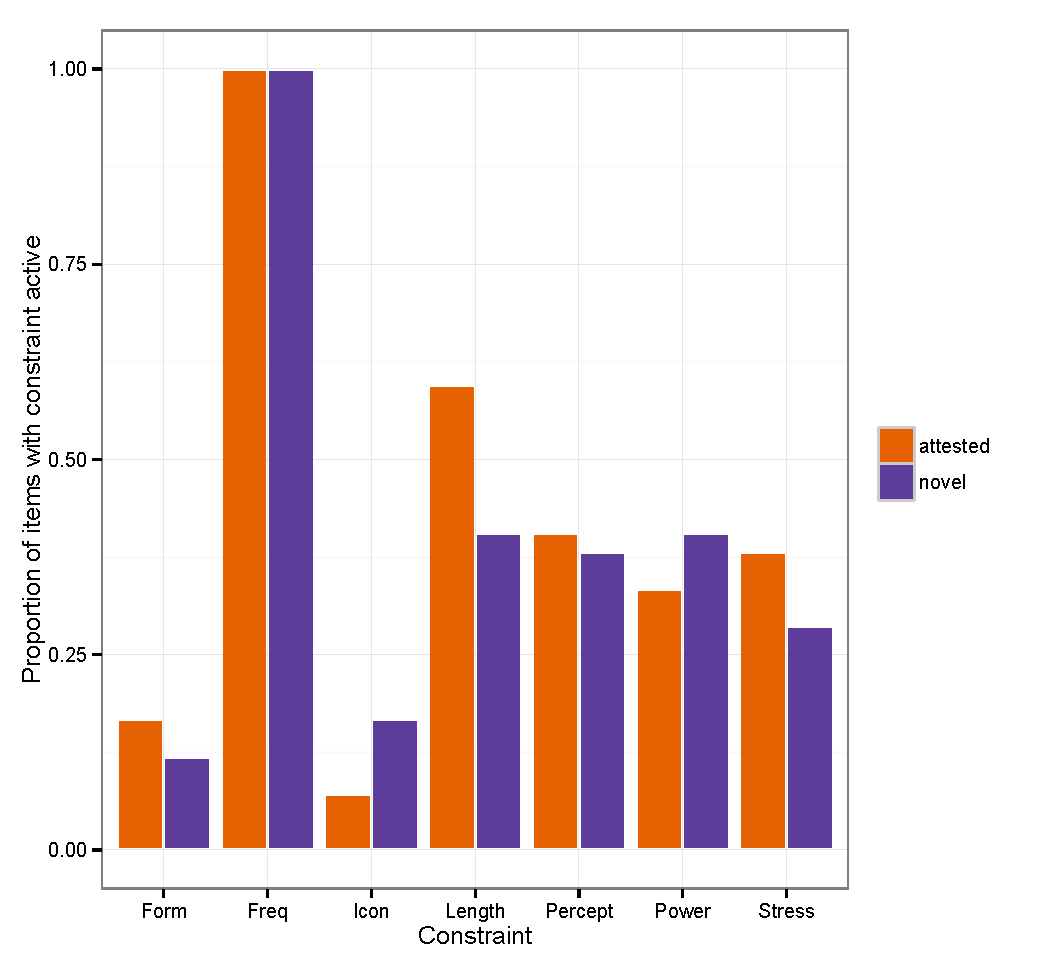
\includegraphics[scale=0.8]{constraint-activity-bar-graph.pdf}
\caption{Proportion of binomial expressions for which each constraint is active.} \label{fig:constraint-activity}
\end{figure}
\begin{table}[!tbp]
\begin{center}
\begin{tabular}{lrrrrrrr}
\hline\hline
\multicolumn{1}{l}{}&\multicolumn{1}{c}{Form}&\multicolumn{1}{c}{Power}&\multicolumn{1}{c}{Icon}&\multicolumn{1}{c}{Percept}&\multicolumn{1}{c}{Length}&\multicolumn{1}{c}{Freq}&\multicolumn{1}{c}{Stress}\tabularnewline
\hline
Form&$ 1.00$&$ 0.22$&$ 0.01$&$ 0.01$&$ 0.01$&$-0.34$&$ 0.02$\tabularnewline
Power&$ 0.22$&$ 1.00$&$ 0.01$&$ 0.06$&$-0.05$&$ 0.05$&$-0.06$\tabularnewline
Icon&$ 0.01$&$ 0.01$&$ 1.00$&$-0.11$&$ 0.44$&$ 0.26$&$ 0.30$\tabularnewline
Percept&$ 0.01$&$ 0.06$&$-0.11$&$ 1.00$&$-0.14$&$-0.10$&$-0.17$\tabularnewline
Length&$ 0.01$&$-0.05$&$ 0.44$&$-0.14$&$ 1.00$&$ 0.30$&$ 0.83$\tabularnewline
Freq&$-0.34$&$ 0.05$&$ 0.26$&$-0.10$&$ 0.30$&$ 1.00$&$ 0.21$\tabularnewline
Stress&$ 0.02$&$-0.06$&$ 0.30$&$-0.17$&$ 0.83$&$ 0.21$&$ 1.00$\tabularnewline
\hline
\end{tabular}
\end{center}
\caption{Correlations of constraint activity for attested binomials.} \label{t:constraint-cor-a}
\end{table}



\begin{table}[!tbp]
\begin{center}
\begin{tabular}{lrrrrrrr}
\hline\hline
\multicolumn{1}{l}{}&\multicolumn{1}{c}{Form}&\multicolumn{1}{c}{Power}&\multicolumn{1}{c}{Icon}&\multicolumn{1}{c}{Percept}&\multicolumn{1}{c}{Length}&\multicolumn{1}{c}{Freq}&\multicolumn{1}{c}{Stress}\tabularnewline
\hline
Form&$ 1.00$&$ 0.09$&$0.02$&$-0.01$&$0.15$&$ 0.44$&$ 0.18$\tabularnewline
Power&$ 0.09$&$ 1.00$&$0.05$&$-0.02$&$0.10$&$ 0.13$&$ 0.11$\tabularnewline
Icon&$ 0.02$&$ 0.05$&$1.00$&$ 0.03$&$0.13$&$ 0.03$&$ 0.04$\tabularnewline
Percept&$-0.01$&$-0.02$&$0.03$&$ 1.00$&$0.24$&$ 0.22$&$ 0.11$\tabularnewline
Length&$ 0.15$&$ 0.10$&$0.13$&$ 0.24$&$1.00$&$ 0.10$&$ 0.50$\tabularnewline
Freq&$ 0.44$&$ 0.13$&$0.03$&$ 0.22$&$0.10$&$ 1.00$&$-0.28$\tabularnewline
Stress&$ 0.18$&$ 0.11$&$0.04$&$ 0.11$&$0.50$&$-0.28$&$ 1.00$\tabularnewline
\hline
\end{tabular}
\end{center}
\caption{Correlations of constraint activity for novel binomials.} \label{t:constraint-cor-n}

\end{table}

\section{Experiment 2 region-by-region analyses}\label{word-by-word}
Here we present region-by-region analyses of the self-paced reading data from Experiment 2. Our goals in these analyses are to replicate the results of \citet{SiyanovaChanturia:2011ep} that attested binomial expressions are read faster in their preferred order, and to demonstrate that this finding extends to novel expressions when categorized into preferred/dispreferred orders on the basis of abstract knowledge. Specifically, we analyze reading times by dichotomizing binomials into preferred/dispreferred conditions, rather than using continous abstract knowledge and relative frequency predictors as in Section \ref{multivariate}. For simplicity of presentation, and because we are not concerned here with comparisons across binomial types, we analyze each type (attested/novel) separately.




Residualization on word length and outlier removal are identical to that reported in Section \ref{multivariate}, except that outlier removal was done for each region and each binomial type separately (because each region within each type is analyzed separately in this section).

For each binomial type and region, we fit a linear mixed-effects regression model with residualized reading times (in milliseconds) as the dependent variable. Our independent predictor of interest is a dichotomous preferred/non-preferred variable (treatment coded with ``preferred'' as the reference level). Details of how preferred order is assessed vary between binomial types and are discussed in more details below. Trial order is also included as a predictor. Following \citet{Barr:2013vf}, we use the maximal random effects structure for subjects justified by the experimental design, namely an intercept and a slope for preferred/non-preferred order. We also include a random by-subjects slope for trial order. For items, defined as unordered word pairs, we use an intercept and a slope for a binary alphabetical/non-alphabetical factor (comparable to that used in Section \ref{multivariate}). Results for the predictor of interest are shown in Table \ref{tab:spr-results}.

% latex.default(spr.table, caption = "Means, standard errors, and t values for coefficient of preferred/dispreferred predictor in the region-by-region analyses of the self-paced reading experiment.",      label = "tab:spr-results", file = "../paper/spr-mean-se",      n.rgroup = rep(2, dim(spr.table)[1]/2), title = "") 
%
\begin{table}[!tbp]
\scriptsize
\caption{Means, standard errors, and \emph{t} values for the estimated coefficient of the preferred/dispreferred predictor in the region-by-region analyses of the self-paced reading experiment. \emph{t} values greater than 2 are taken to be significant.\label{tab:spr-results}} 
\begin{center}
\begin{tabular}{lllllllll}
\hline\hline
\multicolumn{1}{l}{}&\multicolumn{1}{l}{}&\multicolumn{1}{c}{Prelim}&\multicolumn{1}{c}{Word1}&\multicolumn{1}{c}{And}&\multicolumn{1}{c}{Word2}&\multicolumn{1}{c}{Spill1}&\multicolumn{1}{c}{Spill2}&\multicolumn{1}{c}{Spill3}\tabularnewline
\hline
&&&&&&&\tabularnewline
\textbf{Novel}&Mean (SE)&3.02 (2.14)&11.61 (5.16)&8.21 (6.05)&11.18 (4.79)&-1.74 (4.49)&1.03 (2.41)&2.01 (2.71)\tabularnewline
&\emph{t} value&1.41&2.25&1.36&2.34&-0.39&0.43&0.74\tabularnewline
\hline
&&&&&&&\tabularnewline
\textbf{Attested}&Mean (SE)&-2.05 (1.87)&-3.55 (3.34)&7.44 (2.59)&15.26 (3.37)&8.82 (2.40)&2.94 (2.75)&2.90 (1.91)\tabularnewline
\textbf{(corpus freq)}&\emph{t} value&-1.10&-1.06&2.87&4.53&3.67&1.07&1.52\tabularnewline
\hline
&&&&&&&\tabularnewline
\textbf{Attested}&Mean (SE)&-0.12 (1.91)&-3.39 (3.32)&-1.79 (2.78)&5.87 (3.93)&6.12 (2.64)&-2.29 (2.75)&1.84 (2.01)\tabularnewline
\textbf{(model)}&\emph{t} value&-0.06&-1.02&-0.64&1.49&2.32&-0.83&0.92\tabularnewline
\hline
\end{tabular}
\end{center}
\end{table}

\paragraph{Novel expressions}
For novel expressions, we assign each expression a preferred and non-preferred order on the basis of our abstract knowledge model's prediction for ordering preferences. Results are shown in Figure \ref{fig:spr-novel}. As seen in Table \ref{tab:spr-results}, we find significant effects of order at the Word1 and Word2 regions, with preferred read faster than non-preferred.

\begin{figure}[t]
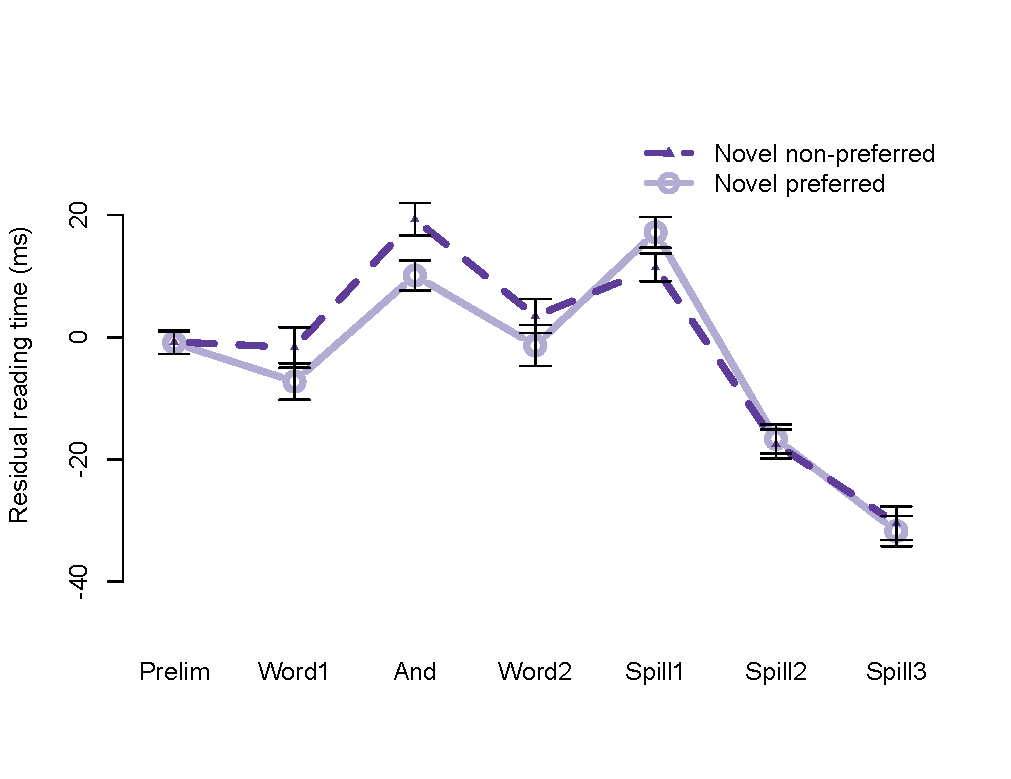
\includegraphics[scale=0.8]{spr-novel.pdf}
\caption{Self-paced reading times for novel expressions. Error bars show standard errors for the predictor of interest (Table \ref{tab:spr-results}).} \label{fig:spr-novel}
\end{figure}

\paragraph{Attested expressions}
For attested expressions, we consider two ways to sort expressions into preferred and non-preferred order: we can use corpus frequencies, replicating \citet{SiyanovaChanturia:2011ep}, or we can use abstract knowledge model predictions for a more direct comparison with the novel expressions. We will show results sorted both ways.

We begin by showing results with preferred/non-preferred determined by corpus frequencies as reported by \citeauthor{SiyanovaChanturia:2011ep}\footnote{\citeauthor{SiyanovaChanturia:2011ep}'s reported preferences differ from the Google n-gram preferences for one item, \emph{family and friends}.}  Results are shown in Figure \ref{fig:spr-attested-sc}. We find significant effects of order at the And, Word2, and Spill1 regions, with preferred read faster than non-preferred.\footnote{ \citeauthor{SiyanovaChanturia:2011ep} only report aggregate reading times, not word by word reading times, so we cannot say whether our results directly replicate exactly where in the sentence these effects appear.}

\begin{figure}[t]
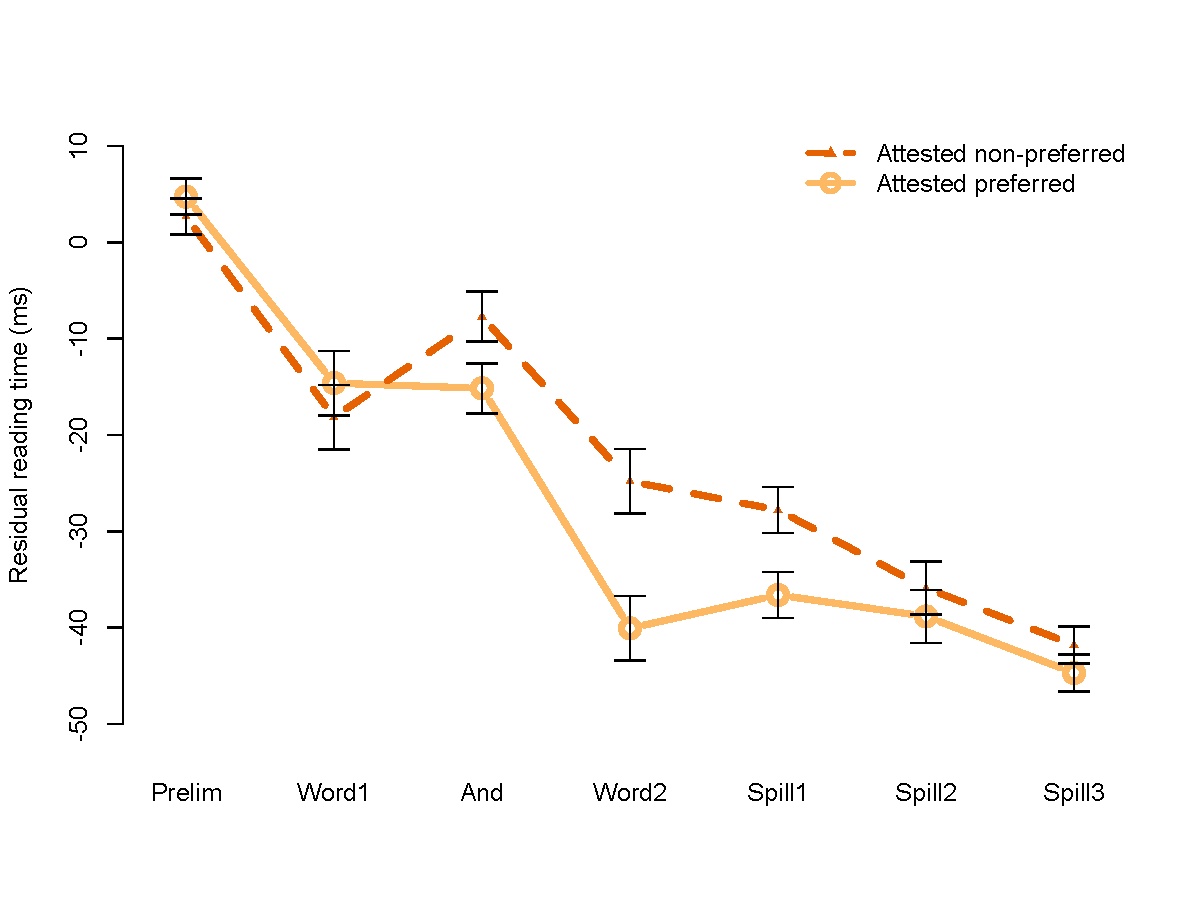
\includegraphics[scale=0.8]{spr-attested-sc.pdf}
\caption{Self-paced reading times for attested expressions with preferred direction determined by corpus frequency. Error bars show standard errors for the predictor of interest (Table \ref{tab:spr-results}).} \label{fig:spr-attested-sc}
\end{figure}

%:
Next we analyze our attested expressions as sorted by abstract knowledge model predictions. Results are shown in Figure \ref{fig:spr-attested-model}. We find a significant effect of order at the Spill1 region, with preferred read faster than non-preferred.

\begin{figure}[t]
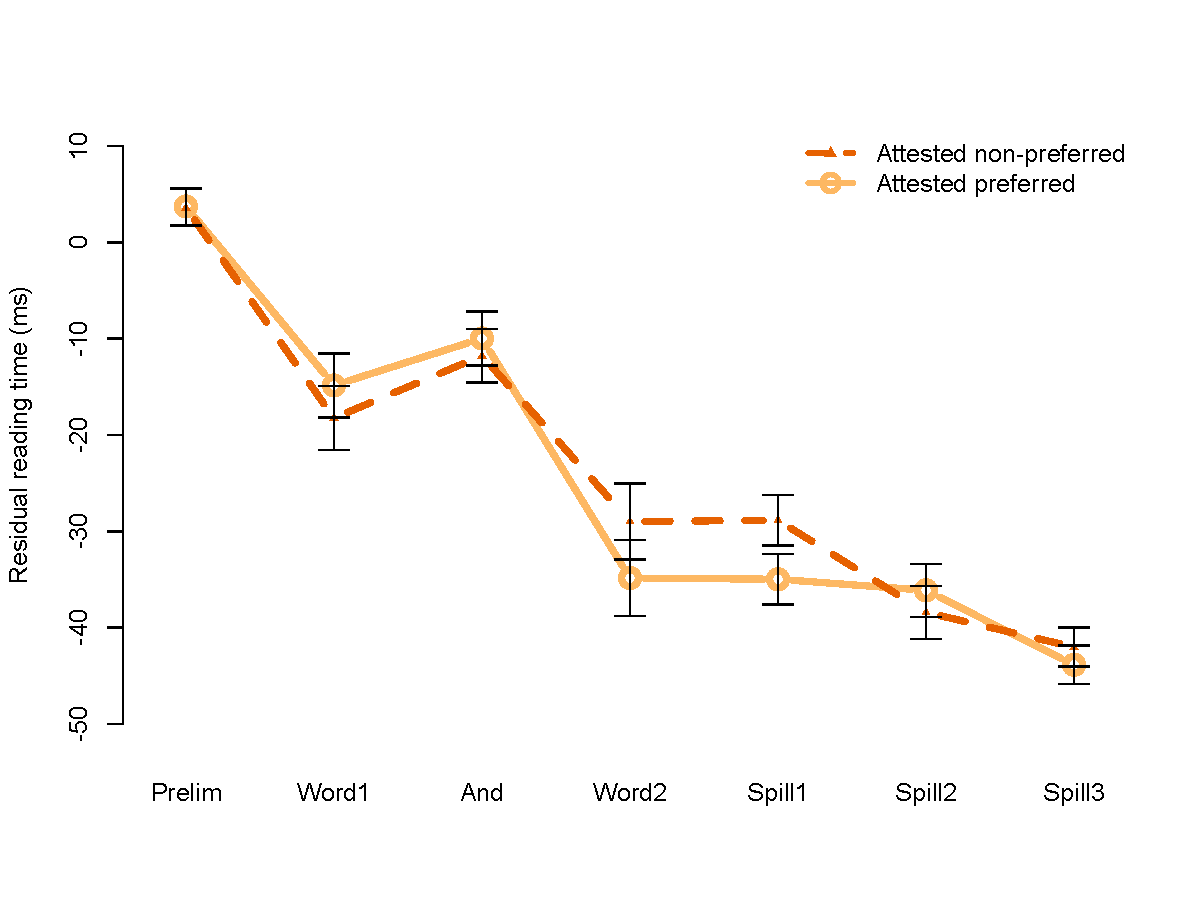
\includegraphics[scale=0.8]{spr-attested-model.pdf}
\caption{Self-paced reading times for attested expressions with preferred direction determined by model predictions. Error bars show standard errors for the predictor of interest (Table \ref{tab:spr-results}).} \label{fig:spr-attested-model}
\end{figure}



\paragraph{Discussion}
We replicate \citeauthor{SiyanovaChanturia:2011ep}'s \citeyearpar{SiyanovaChanturia:2011ep} finding that attested binomial expressions are read faster in their preferred order. We also demonstrate for the first time that novel binomials show online effects of abstract constraints on ordering, with faster reading times in our model's predicted preferred direction.

We do not present a region-by-region version of the multivariate analyses presented in Section \ref{multivariate} because we do not expect the results seen there to hold at each region individually. As noted in Section \ref{multivariate}, the analyses presented there took advantage of the fact that within the six-word region analyzed, participants read the same set of words regardless of order of binomial presentation. Within the word-by-word analyses presented here, however, words differ across conditions: Word1 in the preferred condition becomes Word2 in the dispreferred condition, and vice versa (e.g. ``bishops and seamstresses'' versus ``seamstresses and bishops''). Moreover, recall that effects of lexical frequency are one component of abstract knowledge (Section \ref{model}), such that binomials in preferred order on average have a more frequent word preceeding a less frequent word, while binomials in dispreferred order on average have a less frequent word proceeding a more frequent word. Thus, on the basis of lexical frequency alone, we would expect to see the preferred order read faster around Word1 (or shortly thereafter, due to spillover), and the dispreferred order read faster around Word2 (or shortly thereafter). In other words, on the basis of lexical frequency alone, we would expect to see a local reversal of the effect of abstract knowledge around Word2 (although we expect this reversal to be smaller in magnitude than the overall benefit of conforming to abstract knowledge across the binomial as a whole). This prediction is born out numerically in the Spill1 region for novel binomials, although it does not approach significance.

%\begin{table}[htb]
%\centering
%\begin{tabular}{|c|c|c|}\hline
%& novel & attested \\\hline
%Word1 & 7.32 & 10.46 \\
%Word2 & 5.87 & 10.41 \\\hline
%\end{tabular}
%\caption{Average log frequency for lexical items appearing in Word1 and Word2 slots for expressions in preferred order, with preference determined by model predictions for both novel and attested items.}\label{t:lexfreq}
%\end{table}
%

\section{Experiment 2 results with raw reading times}\label{raw-rts}
Here we replicate the analyses presented in Section \ref{multivariate} with raw rather than word-length-residualized reading times. Model results are given in Table \ref{t:spr-all-raw}. Crucial effects are very similar to those seen in Table \ref{t:spr-all}. In a likelihood ratio test comparing this model to a model with only an additive (non-nested) effect of abstract knowledge, we find a marginally significant difference ($\chi^{2}(1)=3.12, p=0.08$). We attribute the lower significant level here compared to that presented in in Section \ref{multivariate} to presence of extra noise in the raw compared to the residualized reading time data.

\begin{table}[t]
\centering
\begin{tabular}{ l  r  r  r  }
\hline\hline
 & \emph{Estimate} &\emph{Std. Error} & \emph{t value}  \\\hline    
Intercept   &  2246.62   &  41.66   & 53.93\\ 
Type: novel & 204.18 &    28.51  & 7.16\\ 
Abs know (Type: attested)      &   0.72    & 24.97  &  0.03\\ 
Abs know (Type: novel) & -56.81 &     19.88 &  -2.86 \\ 
Rel freq &  -57.46  &   19.98  & -2.88\\ 
Trial order &           -198.11   &   9.46 & -20.95\\\hline 
\end{tabular}
\caption{Model fit for results of Experiment 2 using raw reading times. Effects with $t>2$ are taken to be significant. All VIF $< 1.6$.}\label{t:spr-all-raw}
\end{table}

\bibliography{bib}
\end{document}\emph{}